
\chapter{Shubnikov$-$de Haas oscillations in Bi$_2$Te$_2$Se\label{ch:bts}}

Although topological insulators are supposed to have an insulating bulk that does not conduct, previous transport experiments on the suggested TIs found that most of the TI materials have a large bulk conductivity due to the crystal defects and imperfection. For example, although Bi$_2$Se$_3$ and Bi$_2$Te$_3$ have a simple surface state and a large band gap (on the order of 0.3 eV), their bulk carrier densities can only be reduced to approximate $10^{18} cm^{-3}$ after a large amount of work. Furthermore, the chemical doping method that is used to reduce the carrier densities in Bi$_2$Se$_3$ and Bi$_2$Te$_3$ is likely to reduce to the surface mobility. As a result, the surface current is hard to detect and easily immersed in the overwhelming bulk current. The bulk carriers are usually caused by the intrinsic imperfection of the crystals. For instance, despite of extra Se pressure in the growing environment, a large number of Se vacancies can still be generated in Bi$_2$Se$_3$ and then lead to n-type carriers in the as-grown crystals. Meanwhile, Bi$_2$Te$_3$ is known to have Bi-Te anti-site defects that produce p-type carriers. 

Consequently, the metallic bulk has been a big obstacle to the study of new transport phenomena on TIs. Although there are many proposed transport experiments to search for novel physics on the surface of TIs, they depend on a high-quality surface current and the high carrier density in the bulk has severely hampered the progress. Therefore, it is important to reduce the bulk carriers in order to investigate the surface states on TIs. 

To overcome the difficulty, we grew various TI crystals to suppress the bulk carrier density. Among these crystals, one of the most promising ones is Bi$_2$Te$_2$Se. Since Bi$_2$Se$_3$ is n-type due to the Se vacancies and Bi$_2$Te$_3$ is p-type due to the Bi-Te anti-sites, we believe the combined Bi$_2$Te$_2$Se could have a charge compensation between the n-type and p-type carriers. As a result, Bi$_2$Te$_2$Se is likely to have much fewer bulk carriers. In addition, since Bi$_2$Te$_2$Se is a stoichiometric crystal, the surface mobility won't be sacrificed by the chemical dopants.

In this section,we will discuss our transport results on Bi$_2$Te$_2$Se, a TI compound with a large bulk resistivity (6 $\Omega$cm at 4 K). We have observed prominent Shubnikov-de Haas (SdH) oscillations in Bi$_2$Te$_2$Se, which could be used to detect the surface states out of the bulk signal. A fitting to the oscillations yields a surface mobility ($\mu_s\sim$ 2,800 cm$^2$/Vs), which is much larger than the bulk mobility ($\mu_b\sim$ 50 cm$^2$/Vs). These parameters indicate a high surface to bulk current ratio in Bi$_2$Te$_2$Se and it has a potential to serve as the platform TI material for searching Majorana fermions and  axion electrodynamics.

% include other files for sections of this chapter. These use the 'input' command since each section within a chapter should not start a new page.
% If you want to swap the order of sections, it is as simple as reversing the order you include them. 
\section{Crystal and Band Structure of Bi$_2$Te$_2$Se}
\label{sec:bts:bts-band}

Bi$_2$Te$_2$Se's crystal structure is similar to Bi$_2$Te$_3$, with a tetradymite structure and a rhombohedral unit cell. Its space group is $R\bar{3}m$. As shown in Fig. \ref{BTS_structure}A, compared with Bi$_2$Te$_3$, the Te layer between two Bi layers in Bi$_2$Te$_2$Se is replaced by one Se layer~\cite{Ando10}. Since the Bi-Se bonds are stronger than the Bi-Te bonds, the Bi atoms are more likely to stay on their sites than to exchange the sites with Te atoms. Thus such a structure may reduce p-type carriers caused by Bi-Te anti-sites. Besides, compared with Bi$_2$Se$_3$, there are no two adjacent Se layers in Bi$_2$Te$_2$Se. The lack of Se-Se bonds in could also reduce Se vacancies as the Se-Se bonds are not strong and may produce Se vacancies. As a result, the crystal structure of Bi$_2$Te$_2$Se may reduce both the n-type and p-type carriers intrinsically. 

\begin{figure}[!htbp]
  \begin{center}            
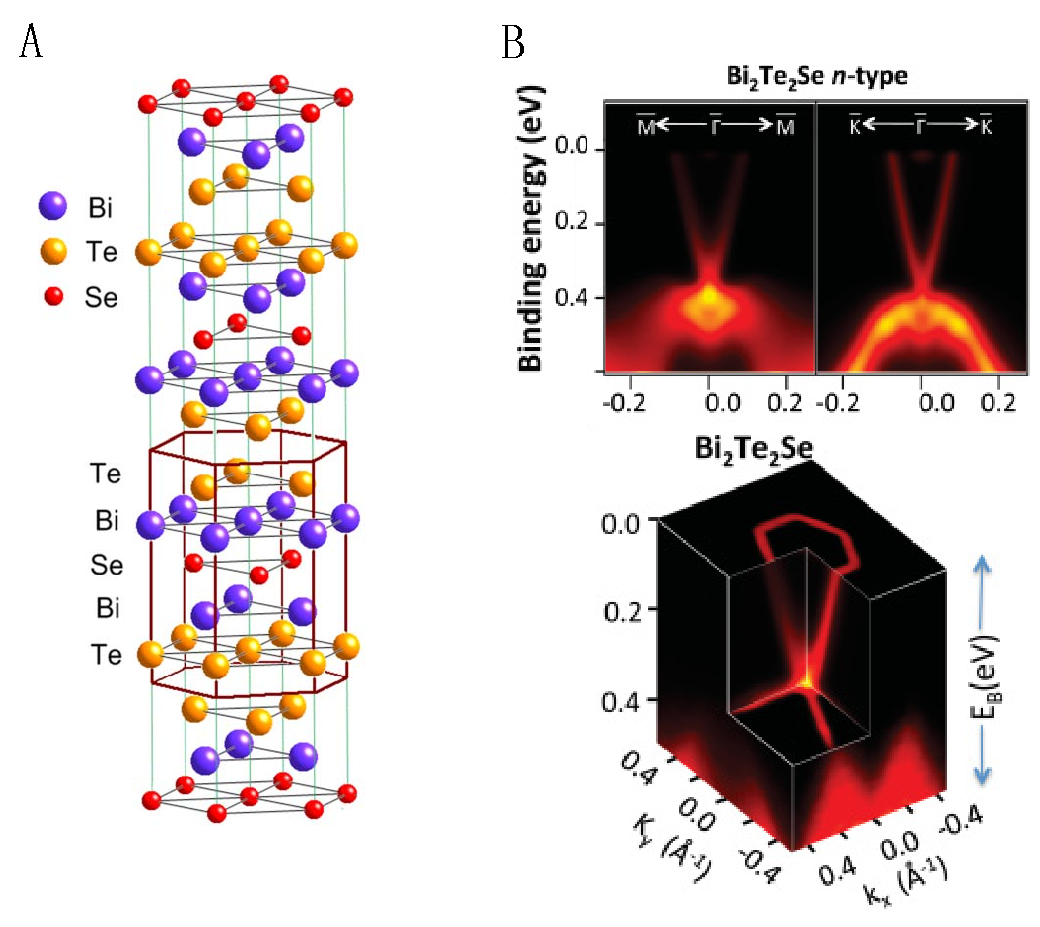
\includegraphics[width=0.9\linewidth]{ch-bts/figures/BTS_structure.pdf} 
\caption{\label{BTS_structure} (Color online) 
The crystal structure and band structure of Bi$_2$Te$_2$Se. (A) The crystal structure of Bi$_2$Te$_2$Se is similar to that of Bi$_2$Te$_3$ with the Te layer between two Bi layers replaced by one Se layer~\cite{Ando10}. (B) The ARPES experiment shows that Bi$_2$Te$_2$Se has a band structure similar to Bi$_2$Te$_3$~\cite{BTS_ARPES}. The band gap is also as large as approximately 0.3 eV, while the surface Dirac point is immersed in the valence band as well.
} 
  \end{center}
\end{figure}

Similar to Bi$_2$Se$_3$ and Bi$_2$Te$_3$, Bi$_2$Te$_2$Se's strong spin-orbital coupling inverts its bulk bands as well. Fig. \ref{BTS_structure}B is the ARPES data on Bi$_2$Te$_2$Se by Hasan's group~\cite{BTS_ARPES}. It demonstrates a clear bulk band gap of approximately 0.3 eV. The V-shape state in Fig. \ref{BTS_structure}B is the spin-polarized single surface Dirac cone. The Dirac point of the surface states is buried in the valence band, as in the case of Bi$_2$Te$_3$.
\section{Experimental Results in the 14T Magnetic Field}
\label{sec:bts:result14T}





%%%%%%%%%%%%%%%%%%%%%%%%%%%%%%%%%%%%%%%%
%%%%%%%%%%%%%%%%%%%%%%%%%%%%%%%%%%%%%%%%
%%%%%%%%%%%%%%%%%%%%%%%%%%%%%%%%%%%%%%%%
%%%%%%%%%%%%%%%%%%%%%%%%%%%%%%%%%%%%%%%% FIGURE 1

%The ARPES experiments by Hasan's group ~\cite{BTS_ARPES} have shown that Bi$_2$Te$_2$Se has a single Dirac cone on the surface. Since Bi$_2$Se$_3$ crystals are $n$-type due to the Se vacancies and Bi$_2$Te$_3$ is $p$-type due to the Bi-Te anti-site defects. We are motivated to grow crystals of Bi$_2$Te$_2$Se so that both dopants could be compensated by each other in order to reduce the total bulk carriers. More specifically, 

To find the composition for optimal compensation, we first grew a series of hybrid semiconductors Bi$_2$Te$_{2-x}$Se$_{1+x}$ and made some test measurements to find the composition that yields the lowest carrier density. The thermopower signal is a good sign for the carrier type, and Bi$_2$Se$_3$ has a negative thermopower and Bi$_2$Te$_3$ displays a positive thermopower. Therefore we also used the thermopower signal to search for the optimal composition. We found that the low-temperature thermopower varies systematically, reflecting changes in $E_F$. 

The first generation of Bi$_2$Te$_2$Se crystals in our experiments were grown by a modified Bridgeman method from high purity elemental starting materials. We heated a mixture of stoichiometric Bi, Te and Se elements for one day at 850 $^{\circ}$C in a clean evacuated quartz tube, the melt was cooled to 500 $^{\circ}$C in a temperature gradient and then it was left to anneal for 2 days before cooling rapidly to the room temperature. To mount the contacts, we carefully cleaved the crystals with a razor blade and got a thin piece with a shiny surface. Then we attached contacts using silver paint, and then loaded the sample into the cryostat. We tried to minimize the time of this process so that the fresh surface experiences minimum hazard from oxidization. For the sample reported here, the crystal thickness is $d$ = 110 $\mu$m, while the distance between voltage leads equals 0.5 mm.  Fig. \ref{figRvsT_lo}A shows the resistivity v.s. temperature profile measured at $B$ = 0. Above 60K, it has a steep increase as the temperature drops, indicating that $E_F$ is in the bulk band gap. Below 40 K, the value of $\rho$ starts to saturate and attains values in the range 5-6 $\Omega$cm, or $\sim$1000 times higher than in non-metallic Bi$_2$Te$_3$. Converted to an areal resistance $R_{\square}= \rho/d$, the low-$T$ resistance corresponds to $R_{\square}$ = 400 $\Omega$. The Hall coefficient $R_H$ below 10 K is negative and implies a very small $n$-type bulk carrier density $n_b\sim 2.6\times 10^{16}$ cm$^{-3}$. From the Hall density and the observed $\rho$ together, we obtain a low bulk mobility $\mu_b\sim$ 50 cm$^2$/Vs.

\begin{figure}[!htbp]
  \begin{center}            
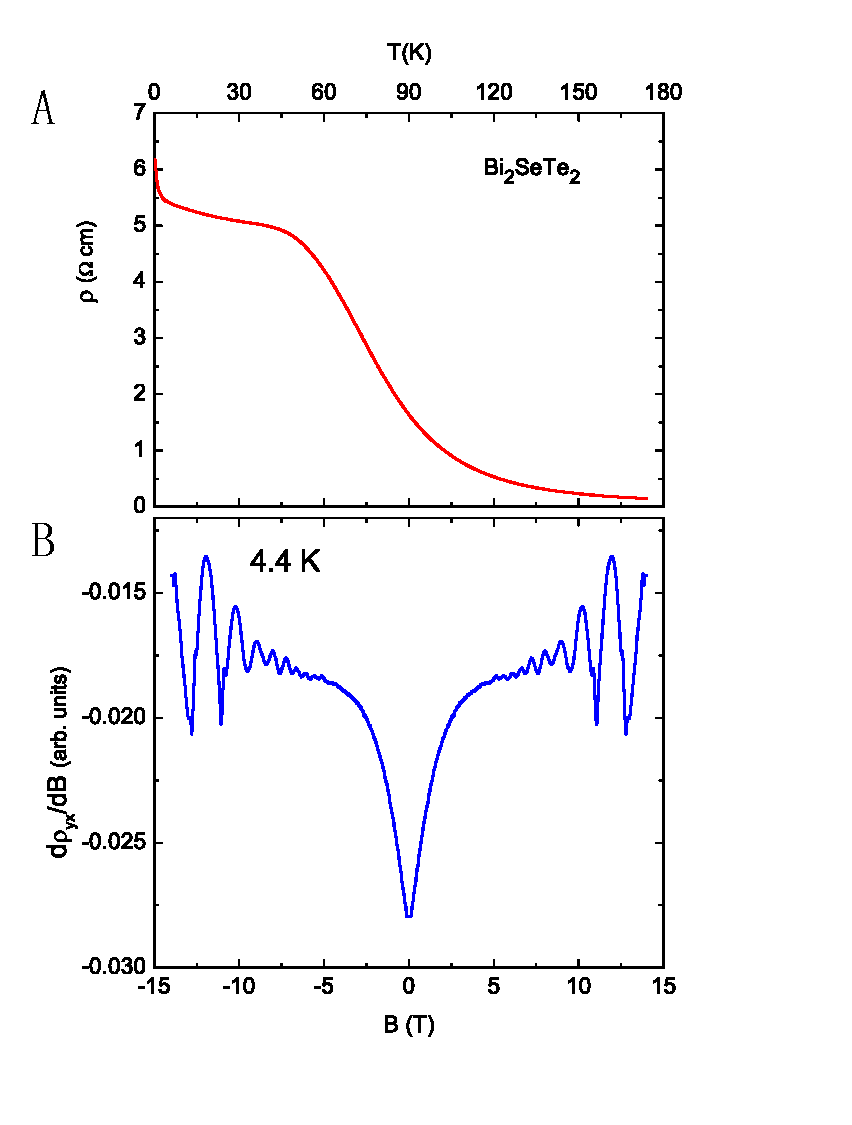
\includegraphics[width=0.9\linewidth]{ch-bts/figures/FigRvsT_lo.pdf} 
\caption{\label{figRvsT_lo}
The resistivity v.s. temperature curve and the derivative of the magnetoresistance curve of the bulk-insulating TI Bi$_2$Te$_2$Se.
Panel (A) shows $\rho$ vs. $T$ measured in $B$ = 0.  Below 10 K, $\rho$ 
reaches as high as 5.5 $\Omega$cm, or an areal
resistance $R_{\square}$ = 400 $\Omega$.  It was one of the most insulating TI crystals. The large resistivity indicates a very low bulk carrier density. Despite the non-metallic
value of $R_{\square}$, sizeable quantum oscillations are observed below 38 K.
Panel (B) displays the prominent SdH oscillations observed 
in the derivative $d\rho_{xy}/dB$ vs. $B$ at 4.4 K. Compared to Bi$_2$Te$_3$, the much larger SdH oscillations in Bi$_2$Te$_2$Se indicate a larger surface proportion of the current in the sample.
} 
  \end{center}
\end{figure}

A powerful way to study the properties of the energy band in a crystal is through the Shubnikovde Haas (SdH) oscillations in the magnetoresistance. High-quality SdH oscillations can uncover a lot of important information, such as the Fermi surface and the mobility of the bands. However, the sample needs to have a high mobility to generate SdH oscillations. In general, a sample with $\mu_b$ as low as 50 cm$^2$/Vs should not display Shubnikovde Haas oscillations in a magnetic field less than 14T. Surprisingly, however, the Hall resistivity $\rho_{yx}$ of our Bi$_2$Te$_2$Se sample displays prominent SdH oscillations that is resolved up to 38 K and down to 5 T. We have detected SdH oscillations in several crystals of Bi$_2$Te$_2$Se with $\rho$-$T$ profiles similar to that in Fig. \ref{figRvsT_lo}A. To emphasize the SdH oscillations, we display the the derivative $d\rho_{yx}/dT$ vs. $B$ at $T$ = 4.4 K in Fig. \ref{figRvsT_lo}B. It clear shows the high quality of the SdH oscillations. Independently, SdH oscillations were also observed in Bi$_2$Te$_2$Se by Y. Ando group~\cite{Ando10}. Since the bulk has a low mobility that could not generate SdH oscillations, we believe that the SdH oscillations originate from the surface states. We will discuss the analysis and reasons below. The work by Ren \etal~\cite{Ando10} also provides solid evidence the surface nature of the SdH oscillations by tracing the Fermi surface area in a tilted magnetic field.

Since the bulk still has a large carrier density, we believe that comparable surface conductance and bulk conductance coexist as parallel charge transport channels in Bi$_2$Te$_2$Se. To separate the bulk and surface contribution in the resistance measurement, it is convenient to convert resistance to conductance for the analysis. Since the total conductance $G$ is additive for parallel channels, the observed conductivity $\sigma_{ij}$ is
then the sum
\be
\sigma_{ij} = \sigma^b_{ij} + G^s_{ij}/d,
\label{eq:sigma}
\ee
where $\sigma^b_{ij}$ is the bulk conductivity and $G^s_{ij}$ is the conductance matrix of the surface states. The conductivity matrix $\sigma_{ij}$ is obtained by inverting the resistivity matrix $\rho_{ij}$. To isolate the SdH oscillations from the surface contribution in $\sigma_{xy}$, we define 
$\Delta\sigma_{xy} = \sigma_{xy} - \langle\sigma_{xy}\rangle$, where $\langle\sigma_{xy}\rangle$ is a smooth background. Here we use a low-power polynomial function to simulate and fit the background curve.


%%%%%%%%%%%%%%%%%%%%%%%%%%%%%%%%%%%%%%%%
%%%%%%%%%%%%%%%%%%%%%%%%%%%%%%%%%%%%%%%%
%%%%%%%%%%%%%%%%%%%%%%%%%%%%%%%%%%%%%%%%
%%%%%%%%%%%%%%%%%%%%%%%%%%%%%%%%%%%%%%%% FIGURE 

\begin{figure}[!htbp]
  \begin{center}            
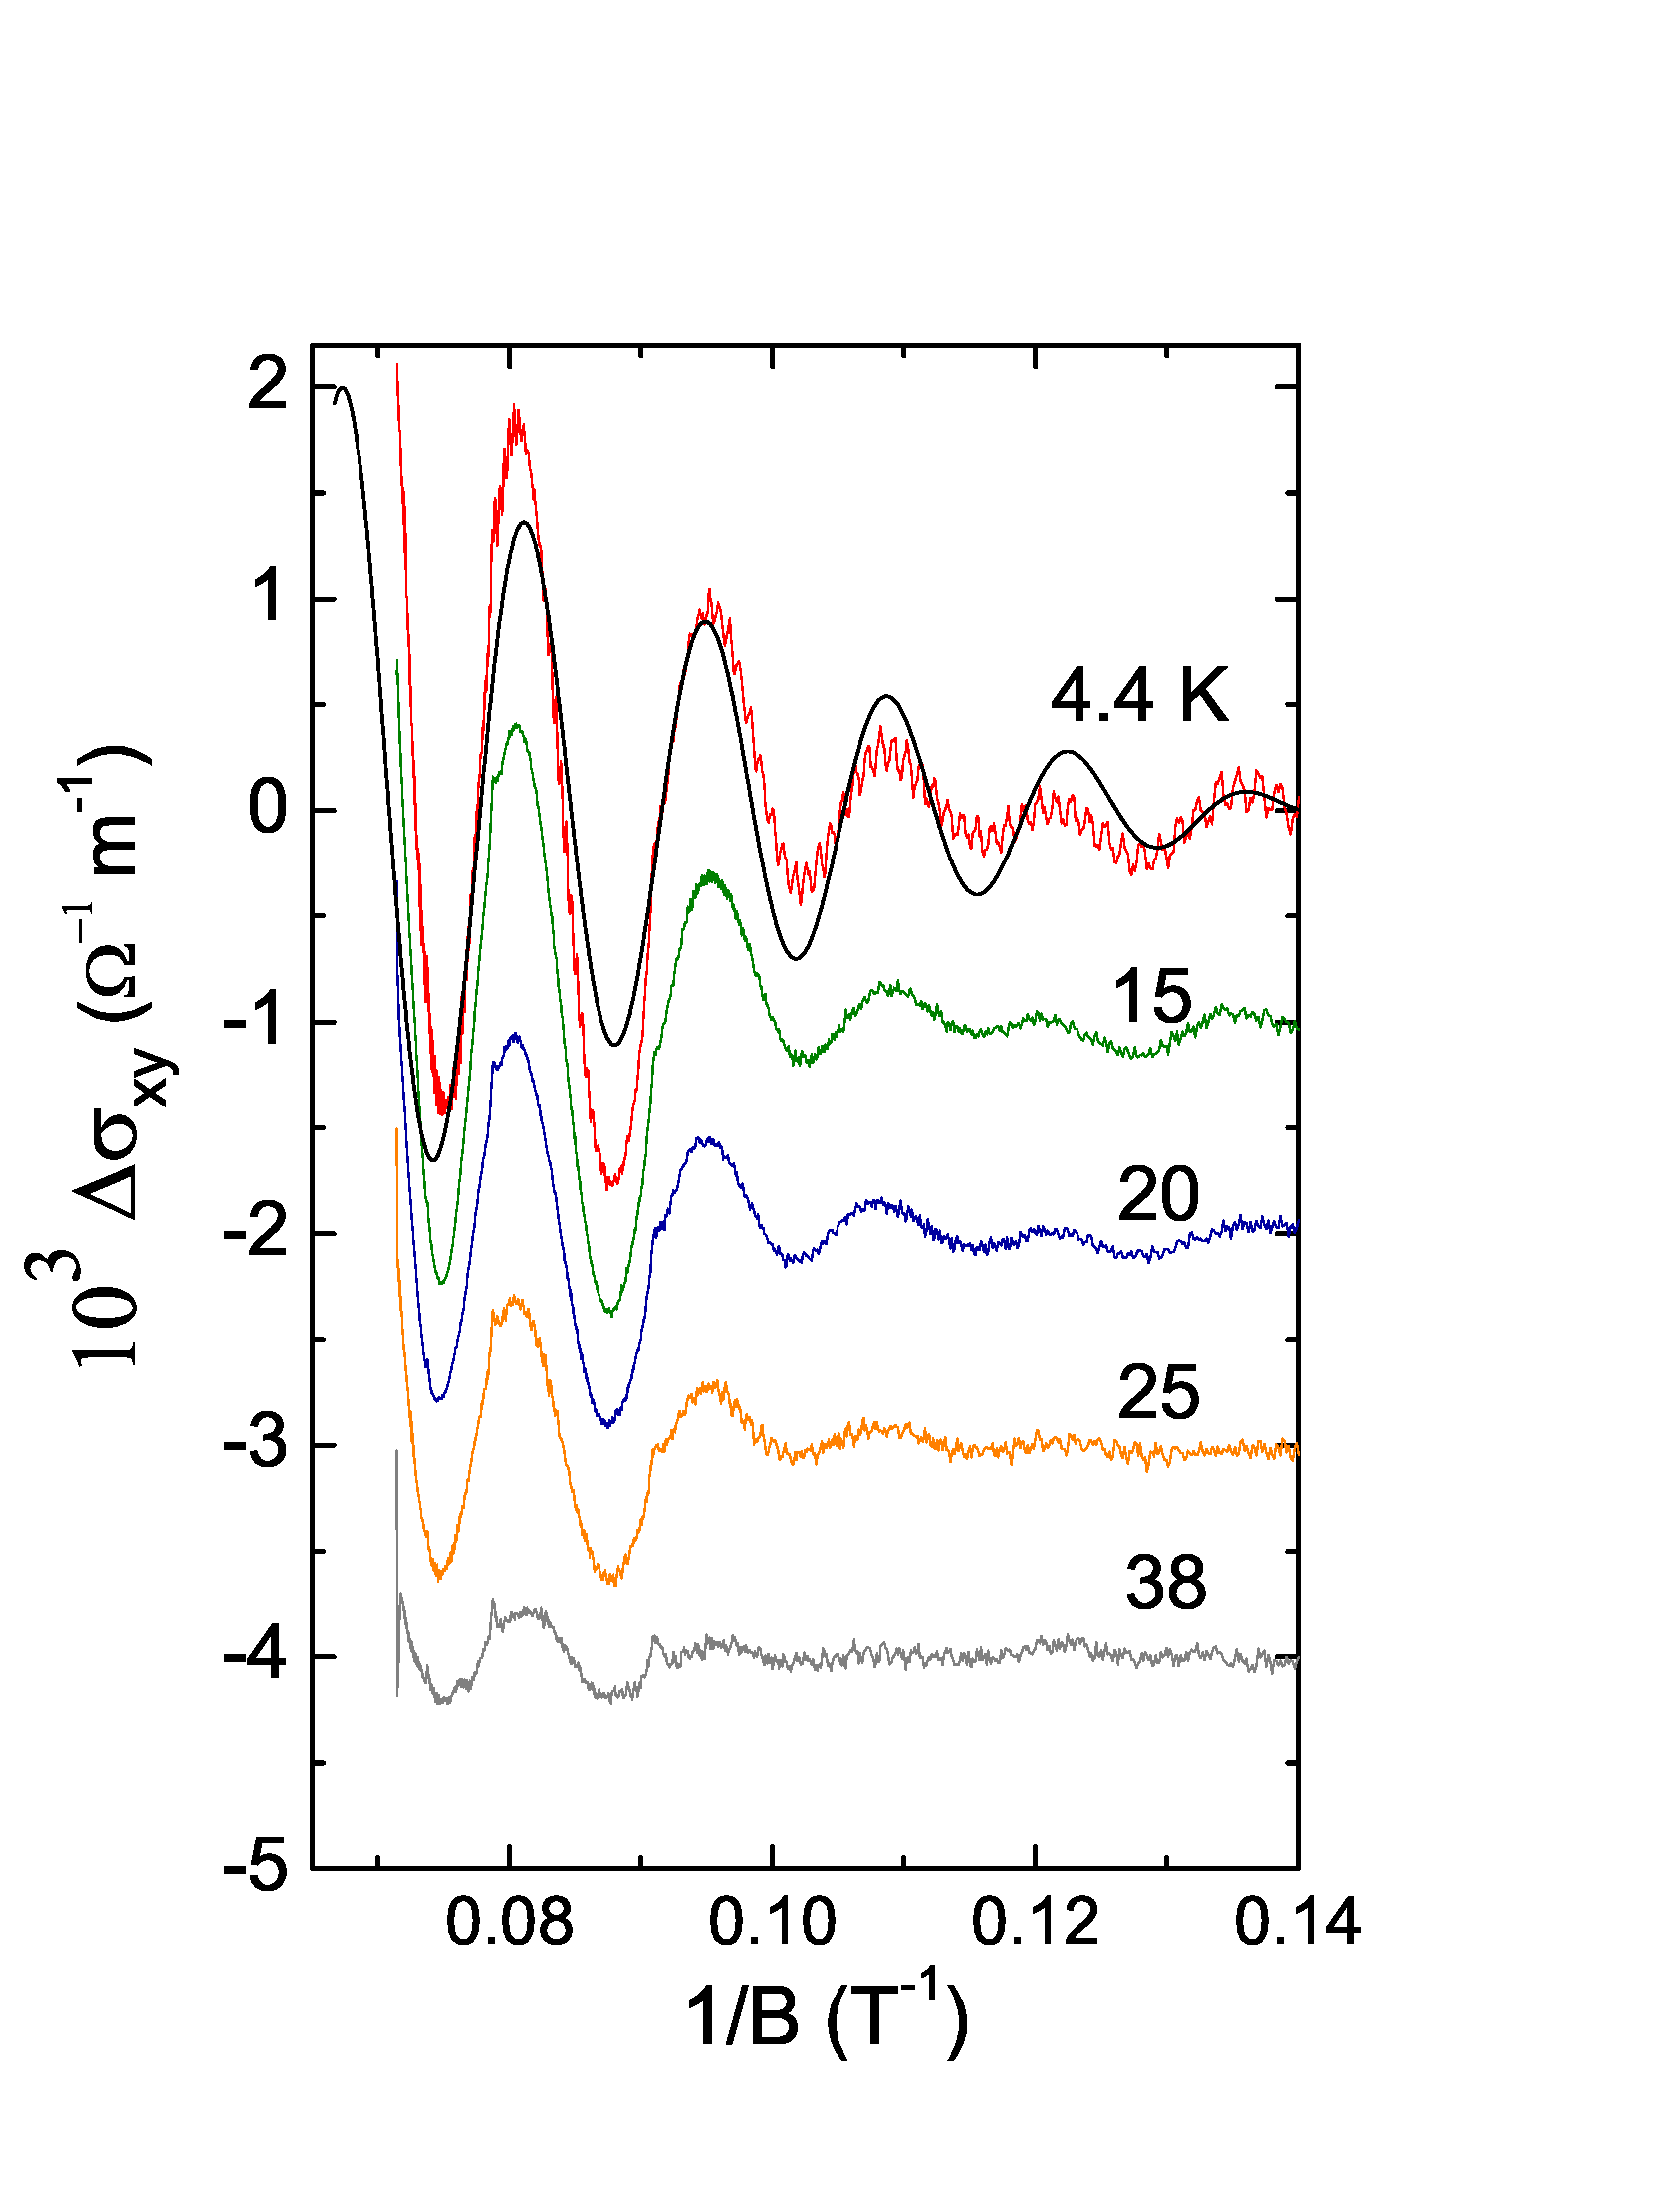
\includegraphics[width=0.9\linewidth]{ch-bts/figures/FigsxyT.eps}
\caption{\label{figsxy} 
Traces of the Hall conductivity $\Delta\sigma_{xy}$ 
(background subtracted) versus $1/B$ at selected $T$ for Bi$_2$Te$_2$Se.
The amplitudes of the oscillations decrease with an increasing $T$ but are still resolvable to 38 K.  
The smooth curve in the uppermost trace is a fit to $\Delta\sigma_{xy}$ by at 4.4 K 
using Eq. \ref{eq:sdh_hall}. The rapid decrease of the oscillation amplitudes for $1/B>$ 0.09 T$^{-1}$
reflects possible interference between 2 terms of similar amplitudes but slightly different
densities ($n_{s1},\;n_{s2}$) = (1.8, 1.7)$\times 10^{12}$ cm$^{-2}$.  
The fit yields the mobility $\mu$ = 2,800 cm$^2$/Vs and $k_F\ell$ = 41.This mobility is much higher than the one we obtained from the $\rho$ and the Hall density. Thus it indicates a different origin from the bulk states.
}
  \end{center}
\end{figure}


%%%%%%%%%%%%%%%%%%%%%%%%%%%%%%%%%%%%%%%%
%%%%%%%%%%%%%%%%%%%%%%%%%%%%%%%%%%%%%%%%
%%%%%%%%%%%%%%%%%%%%%%%%%%%%%%%%%%%%%%%%
%%%%%%%%%%%%%%%%%%%%%%%%%%%%%%%%%%%%%%%% FIGURE

\begin{figure}[!htbp]
  \begin{center}            
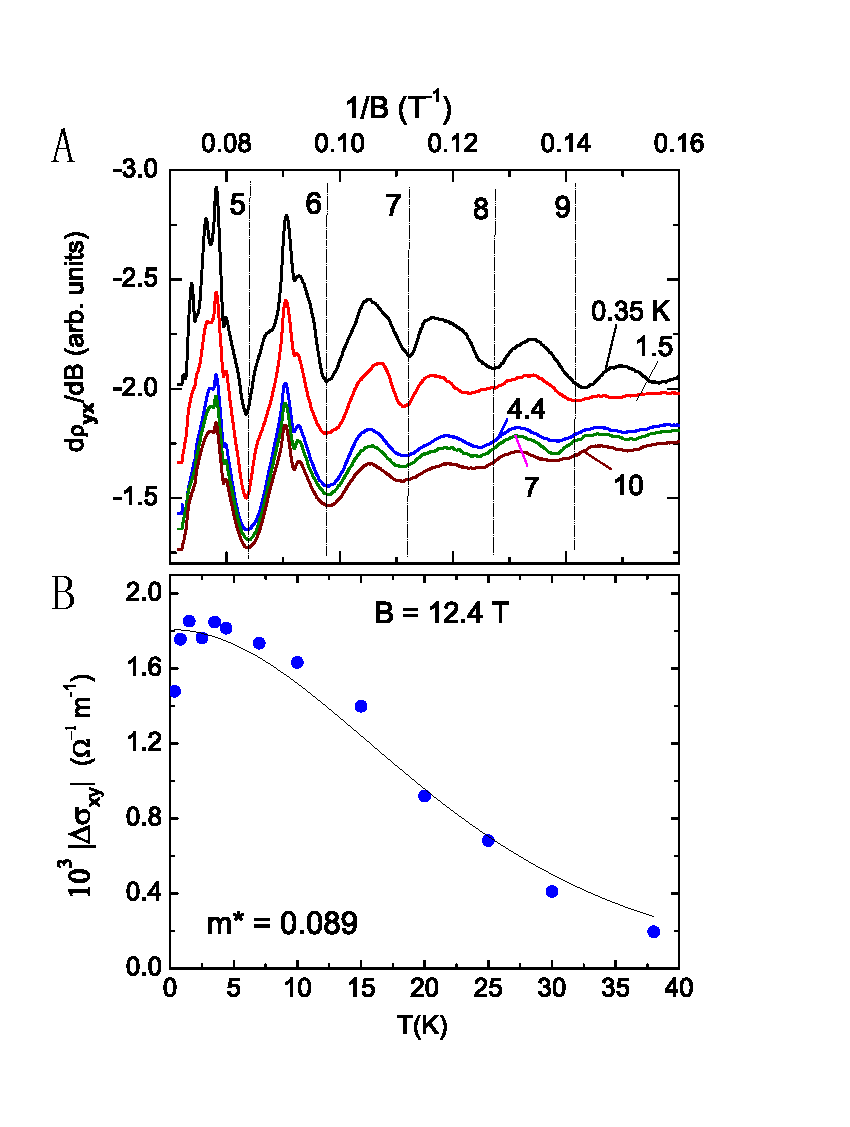
\includegraphics[width=0.9\linewidth]{ch-bts/figures/FigFitvsTemp.pdf} 
\caption{\label{figfit} (Color online) 
Panel (A) displays traces of the Hall resistivity 
$d\rho_{yx}/dB$ in Bi$_2$Te$_2$Se at 5 temperatures.  The minima in $|d\rho_{yx}/dB|$ are used to
fix the index field $B_{\nu}$ (dashed lines with $\nu$ indicated).  
For low LLs with $\nu<$6, there are extra peaks and deeps between the integer fillings, possibly related to some many-body states.
Panel (B) shows the fit of the peak positions versus $T$ with $B$ fixed at
12 T.  The fitting curve is based on Eq. \ref{eq:sdh_hall}. The fit yields $m^*$ = 0.089 $m_0$ (free mass).  With $k_F$ = 0.047 \AA$^{-1}$,
the inferred velocity $v_F$ = 6.0 $\times 10^5$ m/s.
} 
  \end{center}
\end{figure}

We show the background-subtracted conductivity $\Delta\sigma_{xy}$ versus $1/B$ at various temperatures (curves were measured at 13 temperatures in the range 0.3 $\le T\le$ 38 K) in Fig. \ref{figsxy}. On the $1/B$ axis, the oscillations have a clear period which indicates that they are SdH oscillations caused by the Landau level quantization. The SdH oscillations have large amplitudes below 10K, while the amplitudes decreases rapidly as $T$ increases above 10 K as expected by the Lifshitz-Kosevich theory for SdH oscillations.


We also fit the SdH oscillation curves to the standard Lifshitz-Kosevich expression~\cite{Jalan2010} 
\be
\frac{\Delta\sigma_{xy}}{\sigma_{xy}} = \left(\frac{\hbar\omega_c}{2E_F}\right)^{\frac12}
\frac{\lambda}{\sinh\lambda} e^{-\lambda_D}\cos
\left[\frac{2\pi E_F}{\hbar\omega_c}+\phi\right],
\label{eq:sdh_hall}
\ee
with $\lambda = 2\pi^2k_BT/\hbar\omega_c$ and $\lambda_D = 2\pi^2k_BT_D/\hbar\omega_c$,
where $\omega_c$ is the cyclotron frequency and 
the Dingle temperature is given by $T_D = \hbar/(2\pi k_B\tau)$,
with $\tau$ the lifetime.  Compared with
the SdH expression for the conductivity $\sigma_{xx}$, the phase $\phi$ in the 
Hall conductivity is shifted by $\pi/2$.
For the 2D electron gas, we may write the SdH frequency as
$2\pi E_FB/(\hbar\omega_c)$, which simplifies to $4\pi^2\hbar n_s/e$, with the 2D
carrier density $n_s = k_F^2/4\pi$ (per spin).  
As shown in Ref.~\cite{Gusynin2005}, Eq. \ref{eq:sdh_hall} may be employed in a Dirac system
if we write the cyclotron mass as $m_c = E/v_F^2$.  

As shown in Fig. \ref{figsxy}, we notice that it is not possible to get a reasonable fit for the SdH oscillations using one single SdH
frequency, as the SdH oscillation curves seem to have a beating pattern that come from two close frequencies.  For example, at $T<$ 6 K, the sharp decrease of the oscillation amplitudes for the range $B^{-1}>$ 0.12 T$^{-1}$ (the top curve in Fig. \ref{figsxy}) suggests a beating effect between two terms of nearly equal frequencies. Therefore we added another term to Eq. \ref{eq:sdh_hall} that is identical except for a slight difference in $n_s$ to fit the data. The measured curve of $\Delta\sigma_{xy}$ was fitted reasonably well with the 2 terms as shown by the first curve in Fig. \ref{figsxy} (the absolute value of the surface Hall conductance $G_{xy}$ is not known). In our fitting, there are 5 adjustable parameters ($n_{si}$ and amplitude $A_i$, with $i$ = 1,2) and $T_D$ (assumed same for both). The best fit (top curve in Fig. \ref{figsxy}) is obtained with $A_1 = A_2$ and and densities differing by only 5$\%$ [$(n_{s1}, n_{s2})$ = (1.79, 1.71)$\times 10^{12}$ cm$^{-2}$], corresponding to an average Fermi wavevector $k_F$ = 0.047 \AA$^{-1}$. The fit yields $T_D$ = 8.5$\pm$1.5 K, which corresponds to a mean-free-path $\ell$ = 70-100 nm and a surface mobility $\mu_s = e\ell/\hbar k_F$ = 2,800$\pm$250 cm$^2$/Vs. It indicates that the surface mobility $\mu_s$ significantly exceeds the bulk $\mu_b$ by a factor of $\sim$60. By fitting to the decrease of amplitudes with $T$ at a fixed $B$ (12.4 T), we also get the effective mass $m^*$ = 0.089 $m_e$ (Fig. \ref{figfit}B).  Combined with $k_F$, we obtain a Fermi velocity $v_F\sim$ 6 $\times 10^5$ m/s, higher than that in Bi$_2$Te$_3$. This $v_F$ value is consistent with the one for the surface states observed in the ARPES experiment ~\cite{BTS_ARPES}.


We argue that the high mobility here gives strong evidence for the surface nature of the SdH oscillations in Bi$_2$Te$_2$Se. Otherwise if the oscillations were from the bulk states, the SdH period would then yield a 3D Fermi sphere of radius $k_F$ = 0.047 \AA$^{-1}$, or a 3D density of 3.3$\times 10^{18}$ cm$^{-3}$.  The inferred $\mu$ then would imply a 3D resistivity $\rho_b \sim$ 0.7 m$\Omega$cm at 4.4 K. The large discrepancy (factor of 9,000) from the observed value strongly disagree with a bulk origin for the SdH oscillations. Besides, Ref. ~\cite{Ando10} has measured the SdH oscillations of Bi$_2$Te$_2$Se in a tilted magnetic field. The angle dependence of the measured periods show that the implied Fermi surface (FS) is consistent with the behavior of a 2D FS instead of a 3D one.

These evidences make us believe that the SdH oscillations in our Bi$_2$Te$_2$Se samples come from the high-mobility surface carriers. Also since the SdH oscillations of a 2D electron gas only appear when $\bf B$ is perpendicular to the 2D plane, the two periods are likely from the large top and bottom surfaces of the cleaved crystal that are normal to $\bf B$.  Inferred from $n_{s1}$ and $\mu$, we find
that the conductance of each surface is $G_s = \frac12(e^2/h)k_F\ell \simeq$ 0.72 mS (or $R_{\square}\sim$ 1.39 k$\Omega$). As a result, we infer that the surface conductance accounts for $\sim 60\%$ of the observed conductance at 4 K. 




%%%%%%%%%%%%%%%%%%%%%%%%%%%%%%%%%%%%%%%%
%%%%%%%%%%%%%%%%%%%%%%%%%%%%%%%%%%%%%%%%
%%%%%%%%%%%%%%%%%%%%%%%%%%%%%%%%%%%%%%%%
%%%%%%%%%%%%%%%%%%%%%%%%%%%%%%%%%%%%%%%% FIGURE

\begin{figure}[!htbp]
  \begin{center}            
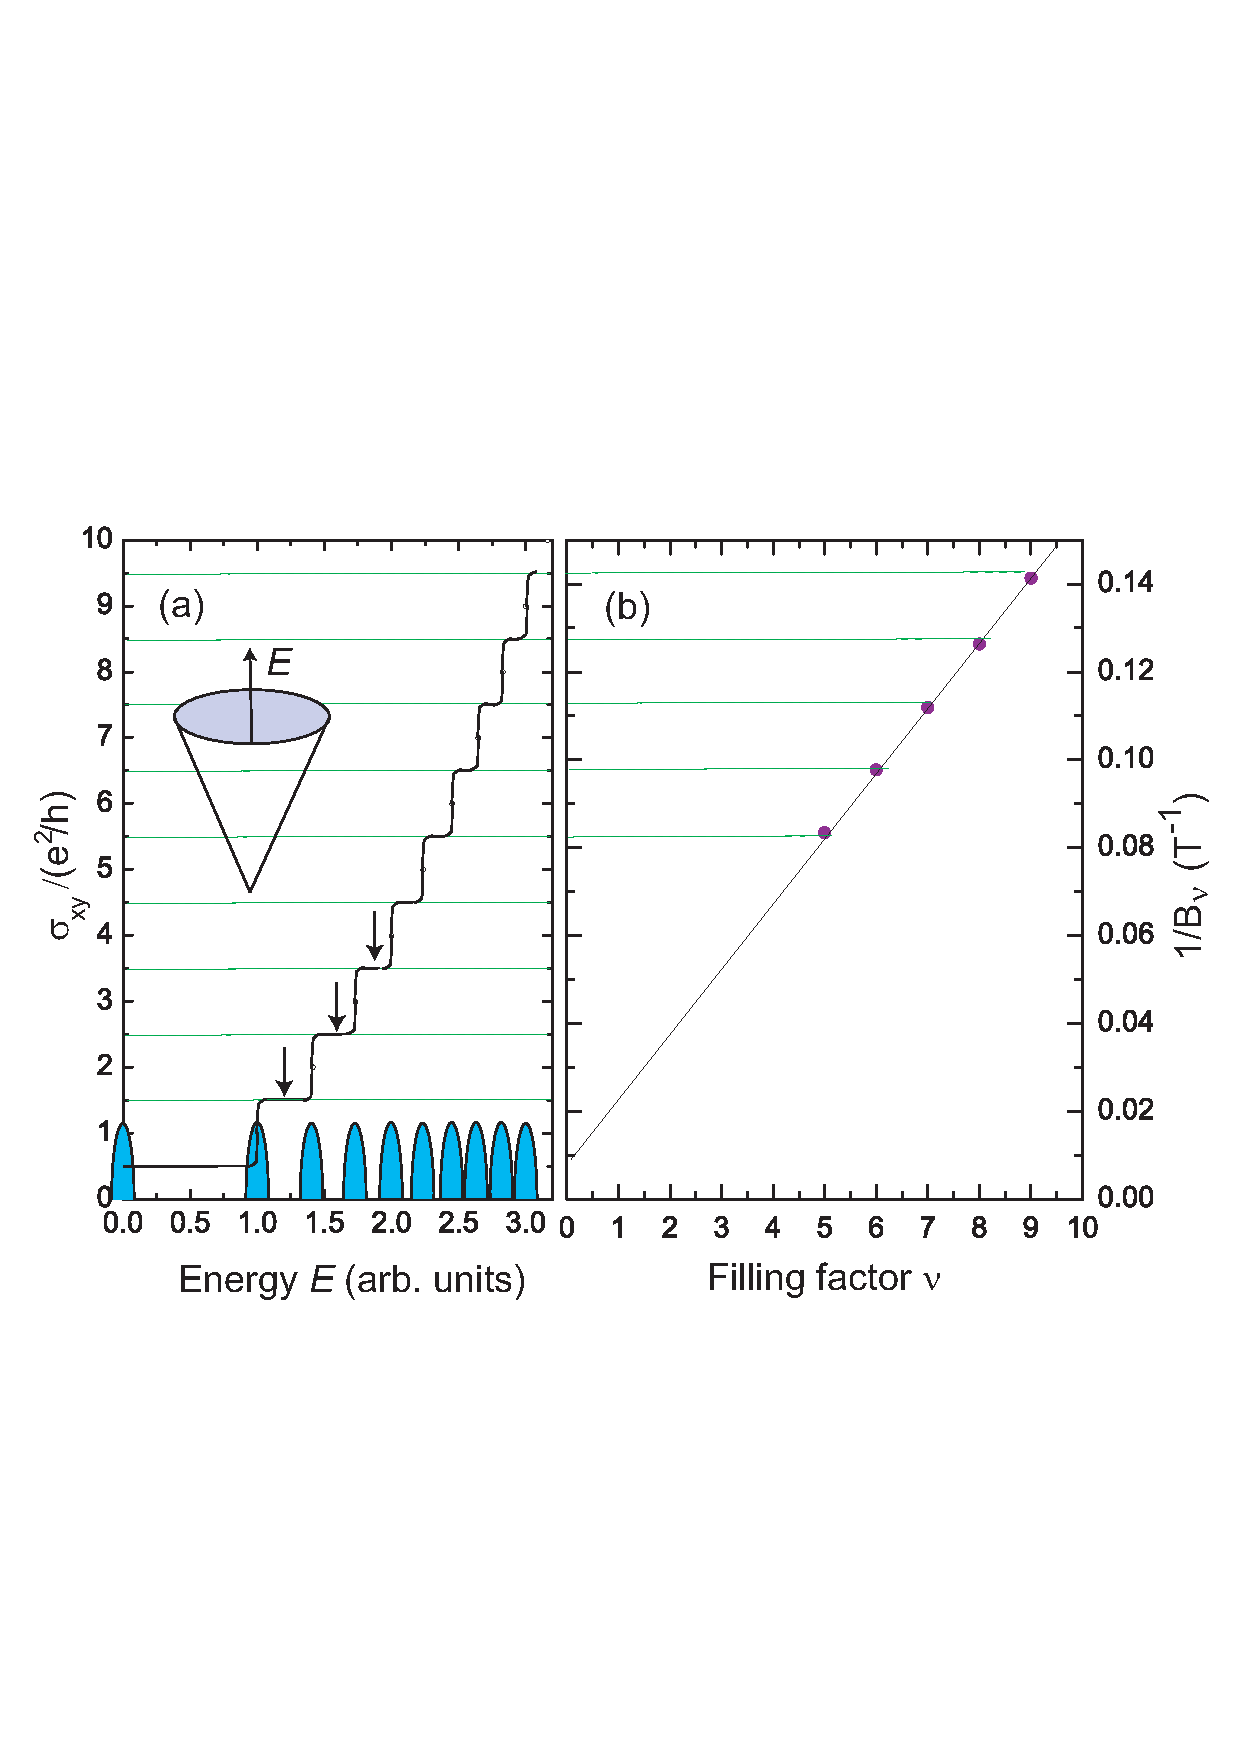
\includegraphics[width=0.9\linewidth]{ch-bts/figures/FigDiracIndex2.pdf} 
\caption{\label{figindex} 
Construction used to fix the filling factors for a Dirac spectrum.  Panel (a) depicts how the Landau indices are decided for a 2D Dirac gas in the quantum Hall regime. It sketches
schematically the step-like increase of $\sigma_{xy} = (e^2/h)[\nu+\frac12]$ versus energy $E$,
where $\frac12$ arises from the $\nu$ = 0 LL at the Dirac point.
The half-ovals are broadened Landau Levels centered at $E_{\nu}=\hbar\ell_B^{-1} v_F\sqrt{2\nu}$.
$B_{\nu}$ are the fields at which $E_F$ falls between LLs (arrows).  The inset
shows the 2D Dirac energy surface in zero $B$.  In Panel (b), we compare this definition of filling factors $\nu$ with
the measured values of $1/B_{\nu}$.
The 5 values of $1/B_{\nu}$ fall on a straight line 
that intercepts the $\nu$ axis at -0.55. The intercept that is close to $\frac{1}{2}$ (mod 1) is consistent with a Dirac spectrum.  
} 
  \end{center}
\end{figure}

Compared to those in Bi$_2$Te$_3$, the SdH oscillations in Bi$_2$Te$_2$Se are much more outstanding. Such prominent oscillations also provide us an opportunity to address whether the surface states' dispersion is Dirac like or not. The previous results on Bi$_2$Te$_3$ have some ambiguity on this issue due to the small amplitudes of the oscillations. In principle, one may plot the
"index" field $1/B_{\nu}$ versus the filling factors $\nu = 1,2 \cdots$, and track the intercept in the limit $B\to\infty$.  Nevertheless, one needs to be careful about whether to take the maxima or minima of $\rho_{xx}$ or $\rho_{yx}$ for the index fields when the sample is not in the quantum Hall regime. Also, as we will discuss in the next subsection, the mixing with a large bulk conductivity will also make this problem even more subtle.  Here we define the index field $B_{\nu}$ as the field at which the chemical potential $E_F$ falls between 2 LLs. The definition could be changed but it should be consistent in $\sigma_{ij}$ and $\rho_{ij}$, and it should agree with the quantum Hall limit as well. With our definition, when the applied field is $B=B_{\nu}$ in the quantum Hall limit, the Hall conductivity has plateau values $\sigma_{xy} = (e^2/h)(\nu+\frac12)$ for the Dirac electrons (compared with $\sigma_{xy} = \nu e^2/h$ for the Schr\"{o}dinger ones). As a result, the index plot n \emph{v.s.} $1/B_{\nu}$ of the Dirac electrons has an intercept of $\frac{1}{2}$ (mod 1) on the $n$-axis, while that of Schr\"{o}dinger electrons intercept 0. In Bi$_2$Te$_2$Se, the large amplitudes could help us determine the "index" field more accurately and thus reduce the uncertainties in the extrapolated intercept.




%%%%%%%%%%%%%%%%%%%%%%%%%%%%%%%%%%%%%%%%
%%%%%%%%%%%%%%%%%%%%%%%%%%%%%%%%%%%%%%%%
%%%%%%%%%%%%%%%%%%%%%%%%%%%%%%%%%%%%%%%%
%%%%%%%%%%%%%%%%%%%%%%%%%%%%%%%%%%%%%%%% FIGURE

\begin{figure}[!htbp]
  \begin{center}            
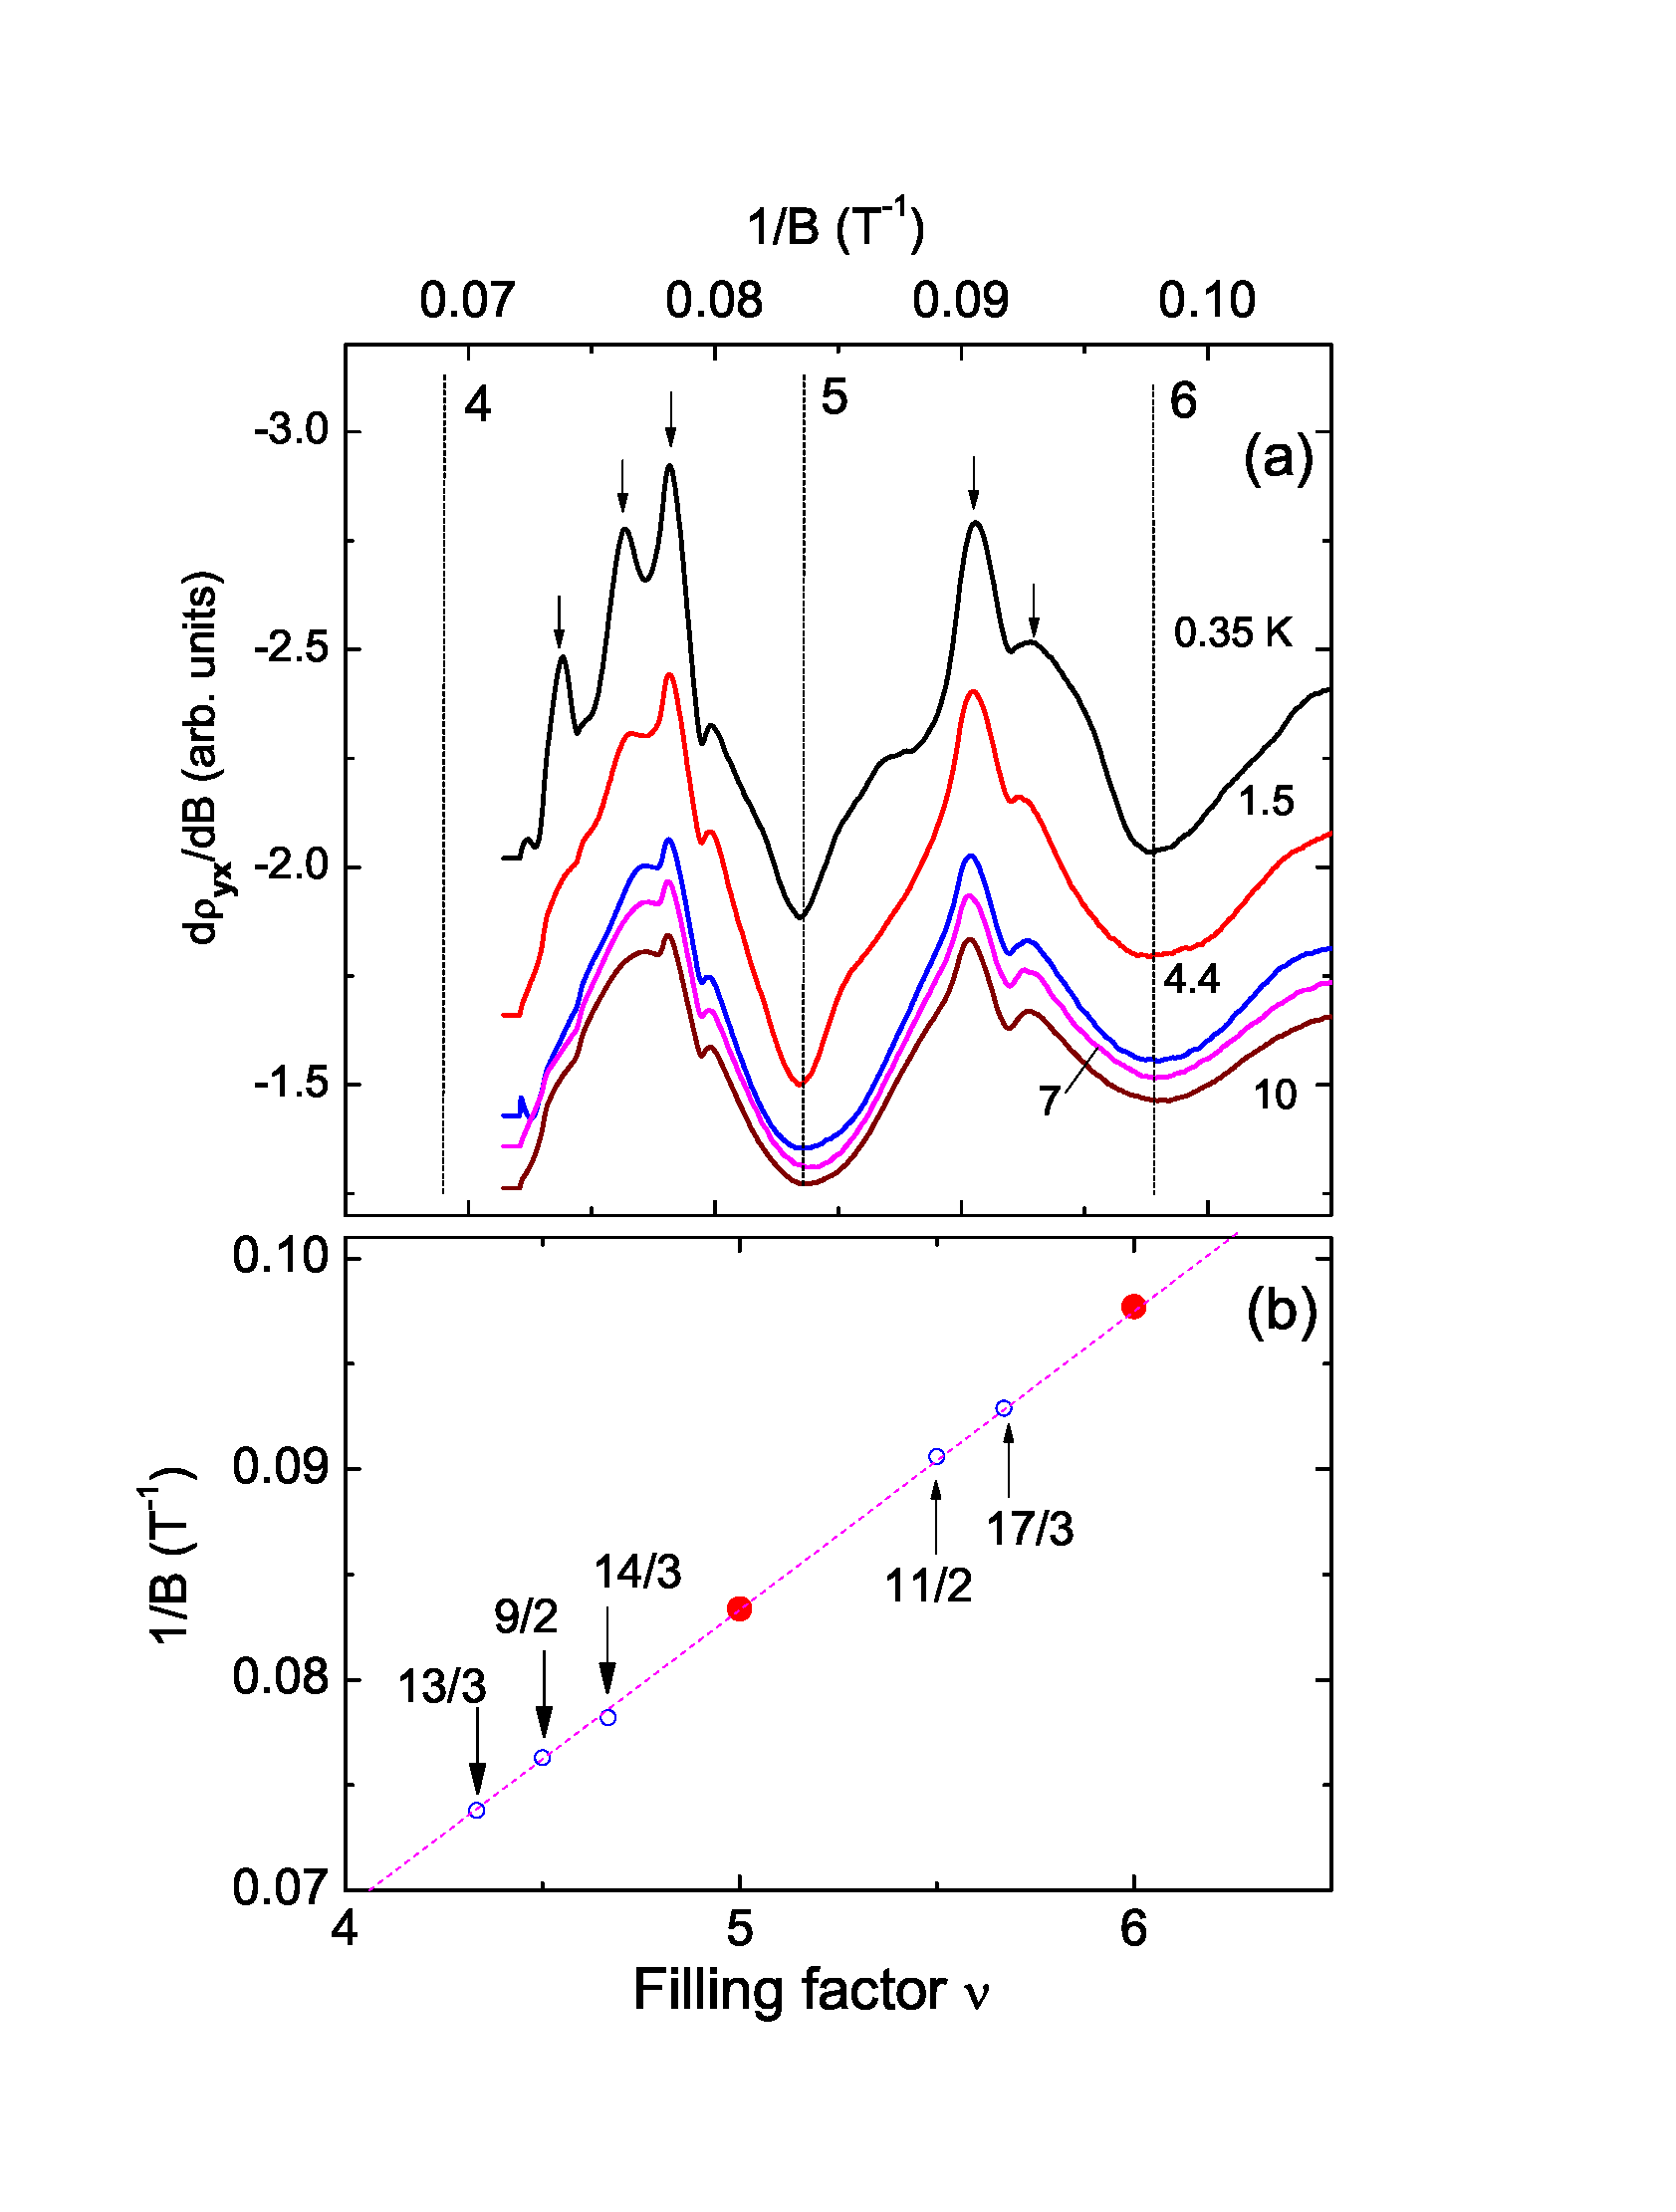
\includegraphics[width=0.9\linewidth]{ch-bts/figures/FigrhoxyExpand.eps} 
\caption{\label{figexpand} 
The possible fractional filling states in the SdH oscillations.
Panel (a): Expanded view of $d\rho_{yx}/dB$ of Bi$_2$Te$_2$Se for 4$<\nu<$6 shows sharp
maxima at non-integer values of $\nu$, at $T$ from 0.35--10 K. The feature decreases rapidly with an increasing temperature. The arrows
locate the more prominent peaks.  In Panel (b), the peak positions plotted
against $\nu$ align well with fractional values of $\nu$ (arrows mark the values
$\nu$ = 13/3, 9/2, $\cdots$, 17/3). 
}
  \end{center}
\end{figure}


Fig. \ref{figindex} is a sketch that relates the index plot ($1/B_{\nu}$ vs. $\nu$) and the Hall plateaus to the Dirac energy spectrum.  
Fig. \ref{figindex}a shows the steps of the quantized Hall conductivity $\sigma_{xy}/(e^2/h)$ versus the Fermi energy $E_F$,  where the shift of $\frac12$ arises from the $\nu = 0$ LL at the Dirac point, as in graphene. The half-ovals drawn on the $E$-axis represent the broadened LLs.  As the density of states (DOS) reaches the peaks at the step-edges of $\sigma_{xy}$, $d\rho_{yx}/dB$ also reaches the maxima. Consequently, the minima in $|d\rho_{yx}/dB|$ locate $B_{\nu}$, the field at which $E_F$ lies between LLs (arrows) as we defined. The $\frac12$-shift of the intercept implies that the line of $1/B_{\nu}$ vs. $\nu$ in Panel (b) does not pass through the origin (whereas it does for a quadratic dispersion).


To find the intercept for our Bi$_2$Te$_2$Se sample, we plot the measured $1/B_{\nu}$ versus $\nu$ in Fig. \ref{figindex}b.
With just one vertical scale adjustment, we can align the 5 data points to the steps in Panel (a).  At our highest $B$, the filling factor is $\nu$ = 5.
The straight line fitted to the data in (b) noticeably intercepts the $\nu$ axis at $\nu$ = -0.55 instead of 0, consistent with the $\frac12$ shift expected from a Dirac spectrum.  

Another possibly interesting point in our data is the additional peaks in the oscillations. Recently, Analytis \etal~\cite{Analytis} reported possibly fractional-filling states in (Bi,Sb)Se$_3$ in very intense fields ($B>$50 T). We also find some similar evidence for fractional-filling states that
emerge at much lower fields (11 T).  Fig. \ref{figexpand}a shows an intriguing array of sharp \emph{maxima} in $d\rho_{yx}/dB$ (arrows) that is apparent for 4$<\nu <$6. The peaks become weaker as $T$ increases from 0.35 K, but some 
are still resolved even at 10 K.  Interestingly, we notice that the peak positions align well with fractional values of $\nu$, as shown in Fig. \ref{figexpand}b. But these fractional features may need more detailed study in samples with higher mobilities. Unfortunately, as we will see in the next subsection, these features do not appear in our samples in a higher magnetic field. Further investigation may needed with samples of higher quality.

\section{Approaching the Lowest Landau Level and Evidence for $\pi$ Berry Phase in 45T}
\label{sec:bts:result14T}
\subsection{Prepare for the High Field Experiments}\label{hifield_intro}
%Everyone needs floating figures in their dissertation. 
%
%As shown in Figure~\ref{fig:pastwork:titlepage}, the Mudd Library dissertation requirements~\cite{muddthesis2009} specify additional options for formatting the title page. For example, if your thesis has multiple volumes, or to indicate the proper formatting for a master's thesis.
%
%\begin{figure}[htb]
%  \begin{center}
%    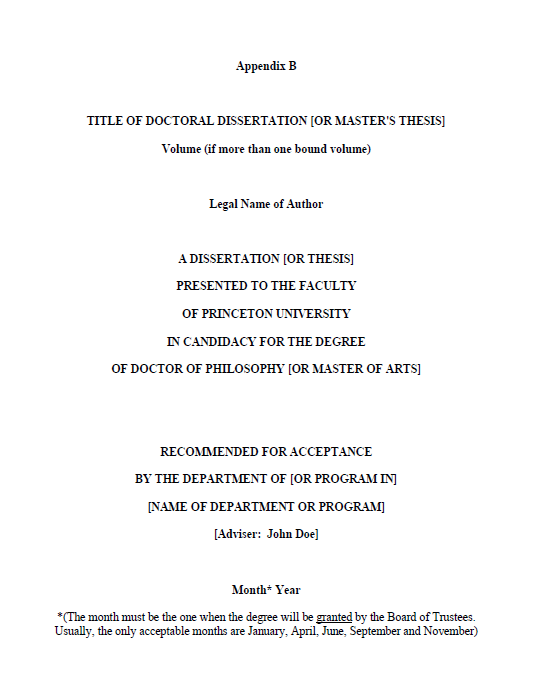
\includegraphics[width=0.9\linewidth]{ch-bts/figures/titlepage}
%    \caption[Sample Title Page Layout]{Sample title page layout~\cite{muddthesis2009}}
%    \label{fig:pastwork:titlepage}
%  \end{center}
%\end{figure}
The 14T data have demonstrated that the surface states on Bi$_2$Te$_2$Se could be well resolved by quantum oscillations due to the large $G^s / G^b$ ratio. However, at 14T, the lowest Landau index of the Bi$_2$Te$_2$Se's surface states is still far away from 0. As a result, the extrapolated intercept of the Landau indices when $1/B\to 0$  is not well resolved. Since the intercept is important for obtaining the Berry phase of the Dirac surface states, it's of great value to approach the lowest Landau level at a higher magnetic field. Besides, the transport experiments close to and at the quantum limit are important for the search of novel interacting physics of the Dirac surface states.

When a strong magnetic field $\bf B$ is applied normal to the surface,
the Dirac states form quantized Landau Levels (LLs) and generate oscillations in the surface conductance $G^s$. To clear any confusion on the symbols, we define the "index field" $B_n$ as the field at which the chemical potential $\mu$ lies between two LLs. This means that the surface states are in the "energy gap" sandwiched by two Landau levels at the field $B_n$. Thus $G^s$ reaches minima at such $B_n$ while the corresponding total resistance $R_{xx}$ reaches maxima if the Hall angle is small as the case here. 
%A plot of the integers $n$ vs. $1/B_n$ gives a nominally straight line with slope equal to
%the FS cross-section $S_F$.  


As we discussed in previous sections, the Landau index plot of $n$ \emph{v.s.} $1/B_n$ will be linear in both Schr\"{o}dinger's case and Dirac's cases. The slope of the fitting line could also give us the Fermi surface cross section $S_F$. The difference between the two cases happens in the limit
$1/B_n\to 0$. In the Schr\"{o}dinger case, there are $n$ filled LLs below $E_F$ when the field equals $B_n$ (as defined).
In comparison, the Dirac electrons have 
$n+\frac12$ filled LLs between $E_F$ and the Dirac point (at $E$ = 0). The extra $\frac12$ Landau level lies right at the Dirac point. It is fixed at the Dirac point because it has equal contributions from both the conduction and valence band, as each contributes half of the states in the $n$ = 0 LL. Therefore, the Landau index line $1/B_n$ vs. $n$ has different intercepts for the Dirac and Schr\"{o}dinger cases. The Dirac electron has an intercept $\gamma = -\frac12$ while the Schr\"{o}dinger electron's $\gamma$ is 0. The additional $\frac12$-shift of Dirac electrons has been confirmed in the quantum Hall effect of graphene~\cite{Kim}. A difference between graphene and the topological insulator is that graphene has four folds of Dirac electrons, while TI only has one for each of the two surfaces.





%%%%%%%%%%%%%%%%%%%%%%%%%%%%%%%%%%
%%%%%%%%%%%%%%%%%%%%%%%%%%%%%%%%%%
%%%%%%%%%%%%%%%%%%%%%%%%%%%%%%%%%% FIGURE 1
\begin{figure}[!htbp]
  \begin{center}
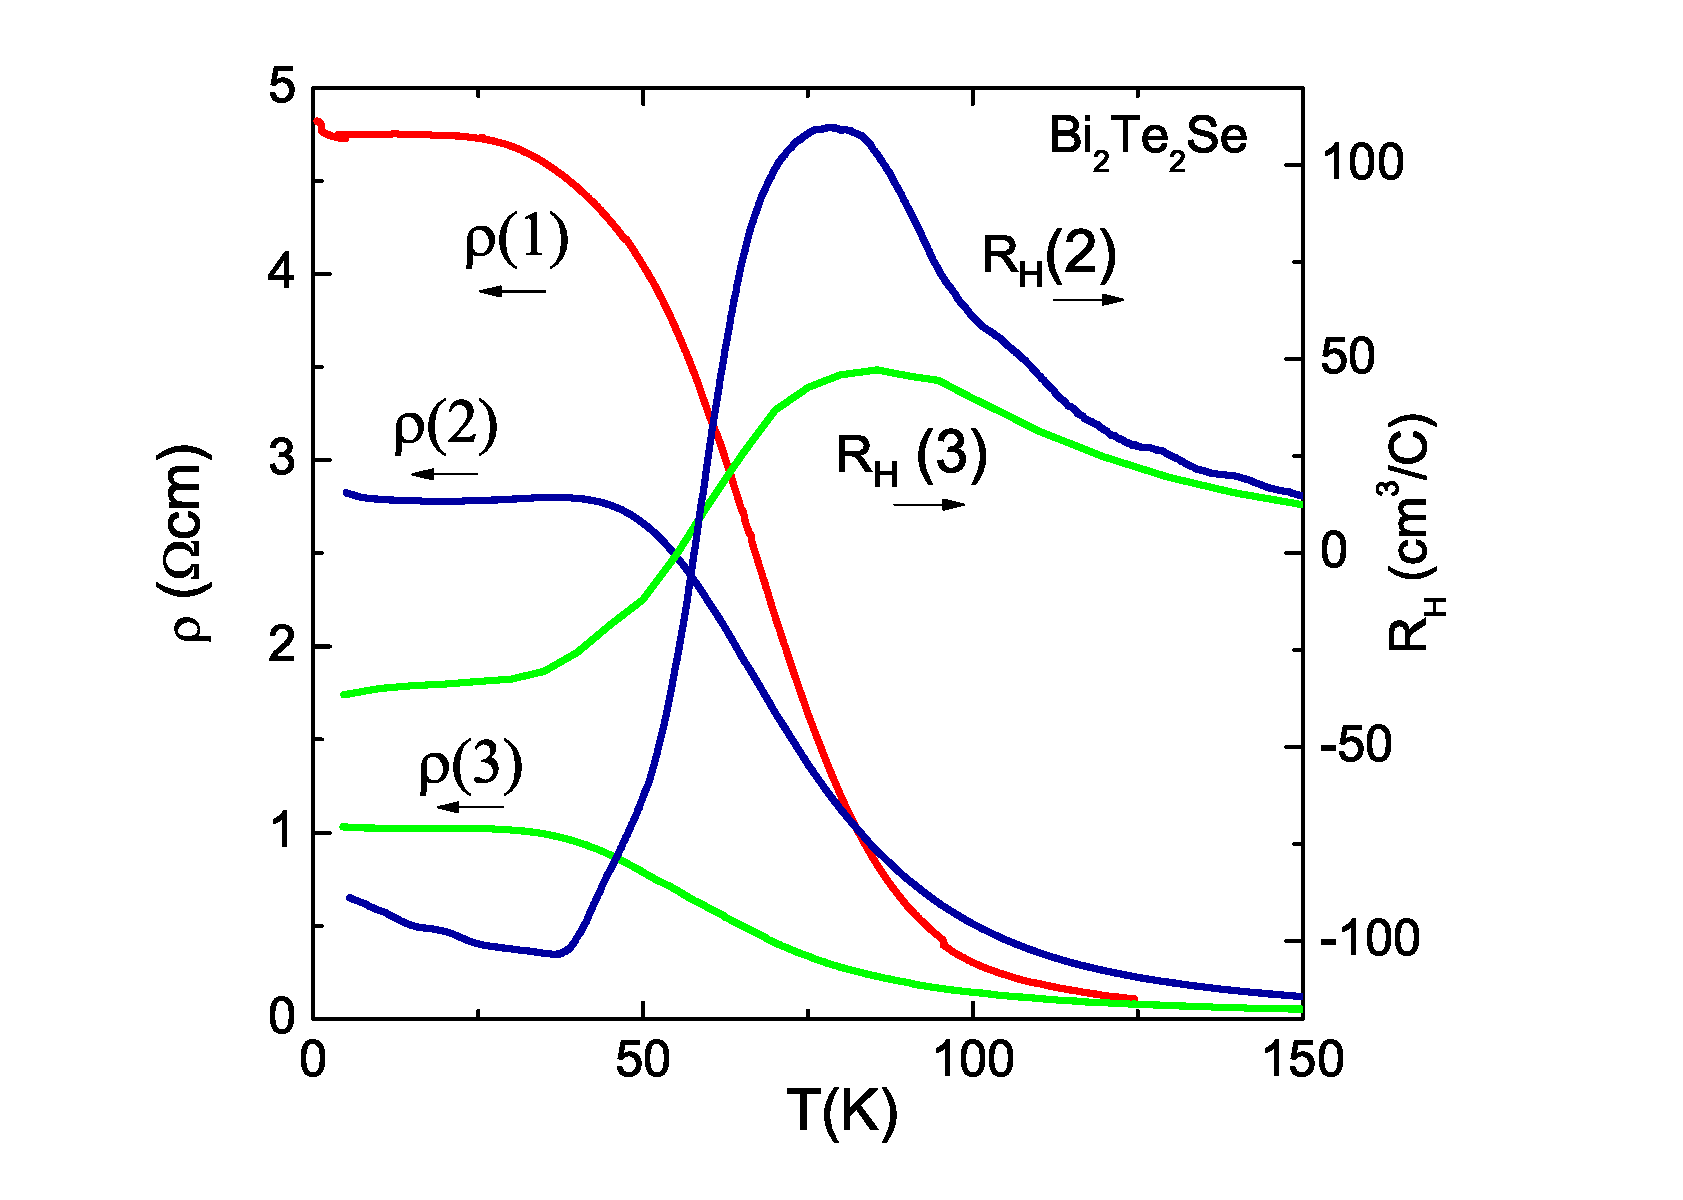
\includegraphics[width=0.9\linewidth]{ch-bts/figures/FigRvsT.eps}
\caption{\label{figRvsT} (color online)
The observed resistivity $\rho$ and Hall coefficient $R_H$ vs. $T$ in Bi$_2$Te$_2$Se for Sample 1, 2, 3. The magnitudes of
$\rho$ and $R_H$ at 4 K vary considerably between annealed samples. But all the samples have an insulating $R-T$ dependence with some $n$-type carriers at 4K. The change in sign of $R_H$ 
near 56 K reflects the thermal activation of bulk hole carriers across a gap of 50 mV.
The largest SdH amplitudes are observed in samples with $\rho >$ 4 $\Omega$cm at 4 K.
}
  \end{center}
\end{figure}
%%%%%%%%%%%%%%%%%%%%%%%%%%%%%%%%%%

Another issue we hope to address here is the Zeeman energy and g-factor of the surface states on Bi$_2$Te$_2$Se. While the strict particle-hole symmetry implies that the lowest Landau level is unshifted in energy, a large Zeeman energy $g\mu_BB$, where $g$ is the surface Lande g-factor and $\mu_B$ is the Bohr magneton, may lead to a high-field distortion of the SdH period and thus a distortion on the Landau index plot. There are some debates on the strength of the Zeeman energy in previous experiments. For example, the in-field STM experiments ~\cite{Hanaguri,Xue10} have shown that the $n$ = 0 LL is unshifted in energy up to 11 Tesla, while Ref~\cite{Taskin} inferred a $g$ factor as large as 76 from the low-field SdH oscillations in transport experiments. Some other quantum oscillation experiments~\cite{Qu,Analytis} had limited resolution due to the bulk contribution. Here we could explore this issue in SdH experiments at a much larger $B$ and with a lower Landau index. The low bulk carrier density in Bi$_2$Te$_2$Se also increases our resolution.

\subsection{Resistivity maxima or minima?}\label{maxmin}
As we mentioned above, the index field $B_n$ plays the key role in determining the intercept shift and the Berry phase in the Landau index plot. While the case for an ideal two-dimensional electron gas(2DEG) is clear in quantum Hall effect, it is important to discuss this issue when the surface and bulk carriers coexist and both contribute a large portion of the total conductance. In the current Bi-based 3D topological insulators, the bulk electrons or holes provide a current channel parallel to that of the surface states. By contrast, the current carried by the 2DEG in graphene and GaAs heterostructures is not mixed with any bulk channels. Thus when $E_F$ falls between two adjacent LLs in the QHE regime of graphene, both the 2D longitudinal conductance $G_{xx}$ and resistance $R_{xx}$ attain a deep minimum (this follows from $R_{yx}\gg R_{xx}$) while $G_{xy}$ and $R_{yx}$ reach finite quantized values. 


%The index field $B_n$ clearly plays the key role in pinning down the -$\frac12$ shift in the index plot. 
%Here we wish to discuss the question of determining $B_n$ when surface and bulk carriers co-exist~\cite{Fu}. 
%In the bismuth-based systems (and other 3D topological insulators), 
%the two-dimensional electron gas (2DEG) on the surface is in intimate contact 
%with bulk electrons which conduct a significant fraction of the 
%applied current. By contrast, the entire current is carried by the 2DEG in graphene 
%and GaAs heterostructures. When $E_F$ falls between adjacent LLs in the QHE regime of graphene, 
%both the 2D conductance $G_s$ and resistance $R_{xx}$ attain 
%a deep minimum (this follows from $R_{yx}\gg R_{xx}$). 


However, the situation becomes subtle when a large
bulk conduction channel exists in parallel (as the case here). The observed conductance matrix
becomes the sum of both the bulk and the surface part, i.e.
\be
G_{ij} = G^s_{ij} + G^b_{ij},
\label{eq:G}
\ee
where $G^b_{ij}$ is the bulk conductance matrix. In Bi$_2$Te$_2$Se, the bulk carriers have a very low mobility ($\mu_b$ ~ 50 cm$^2$/Vs), therefore they do not contribute to the quantum oscillations even at 45T. The additivity of the conductances in Eq. \ref{eq:G} implies that the index fields $B_n$ we defined still correspond to minima in $G_{xx}$. However, due to the large amount of bulk carriers, the bulk $G^b_{xx}$ is dominant. Since $G^b_{xx}$ has a gentle field dependence, the observed resistance now reaches maxima at $B_n$, since $R_{xx} = G_{xx}/[G_{xx}^2+G_{xy}^2]\sim 1/G_{xx} = 1/(G^b_{xx}+G^s_{xx})$. Hence it is less confusing to use the conductance tensor $G_{ij}$ to find the index field $B_n$ because the bulk and surface contribution are additive. We will use this paradigm to analyze our experimental results below. 

When the Hall resistance is not available, as in many experiments, one may still use the SdH oscillations in the longitudinal resistance $R_{xx}$ along, provided $B_n$ is identified with its \emph{maxima}. It is equivalent to converting $R_{xx}$ into $G_{xx} \sim 1/R_{xx}$ if the Hall signal is small compared to $R_{xx}$. It is important to take such care in determining the real index intercept of TI's quantum oscillations, because if people otherwise mistakenly identify $B_n$ with \emph{minima} in $R_{xx}$, a spurious -$\frac12$ intercept will appear for carriers with a Schr\"{o}dinger dispersion.




%%%%%%%%%%%%%%%%%%%%%%%%%%%%%%%%%%
%%%%%%%%%%%%%%%%%%%%%%%%%%%%%%%%%%
%%%%%%%%%%%%%%%%%%%%%%%%%%%%%%%%%% FIGURE 2
\begin{figure}[!htbp]
  \begin{center}
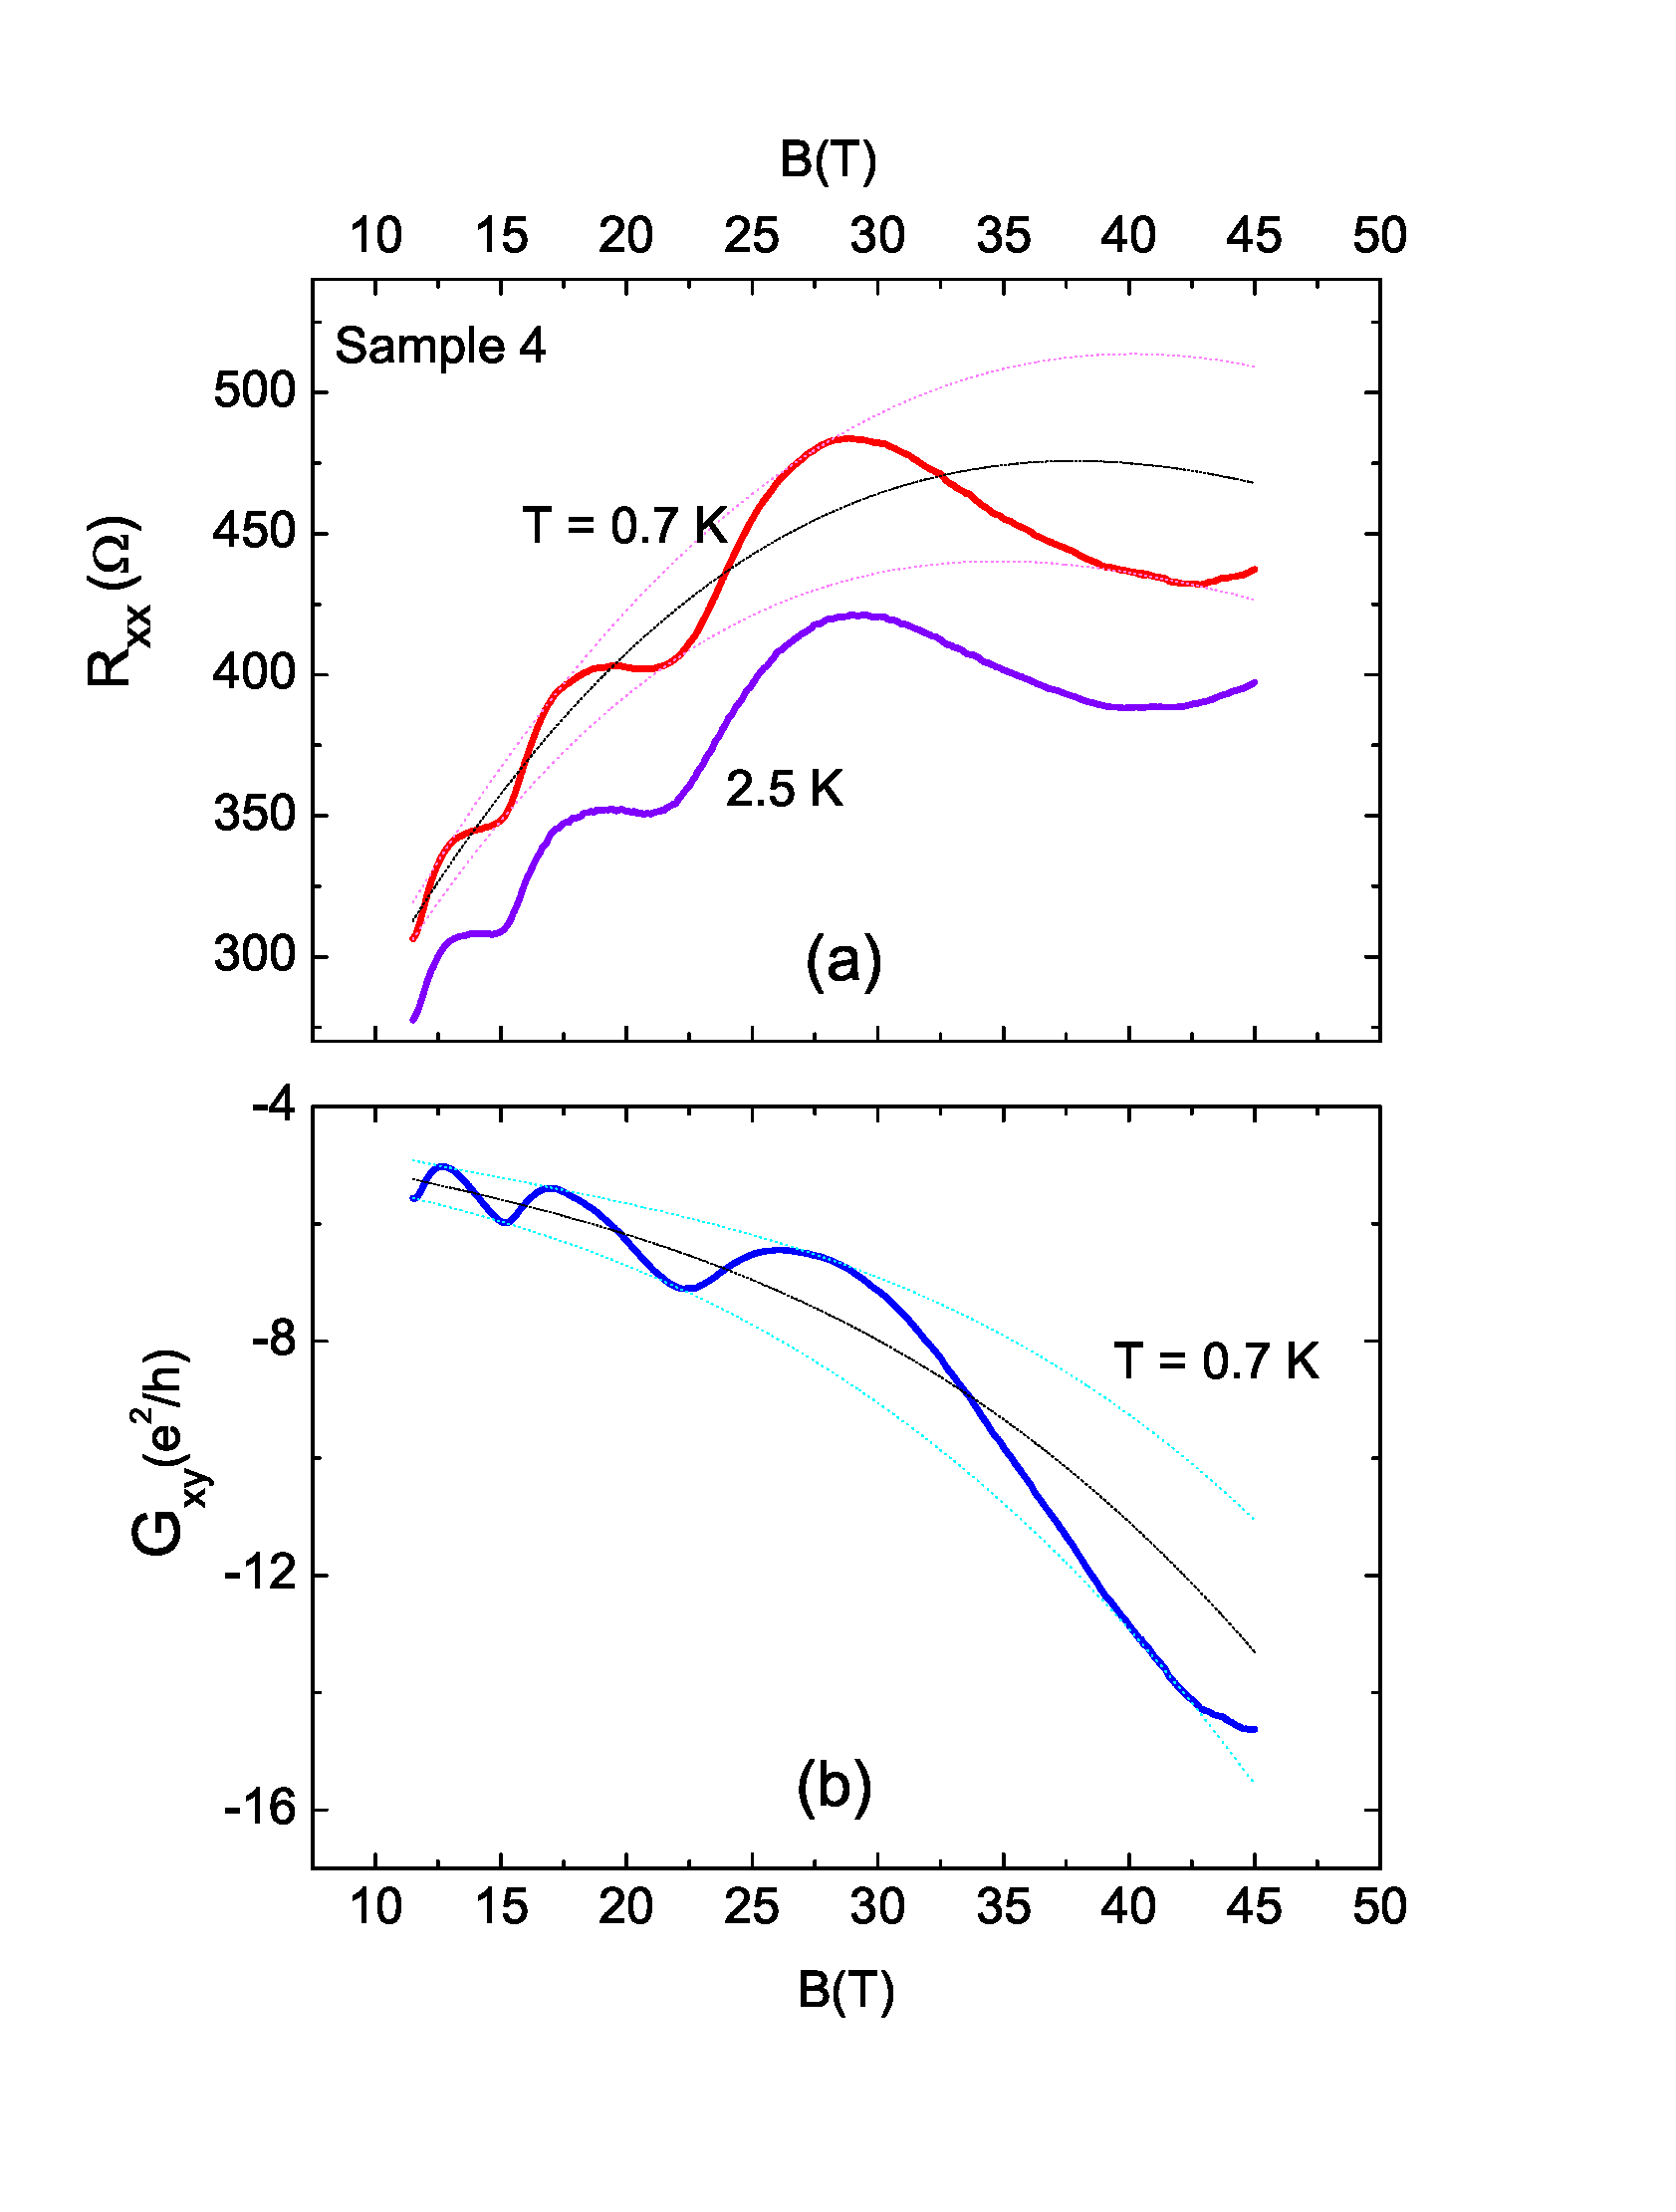
\includegraphics[width=0.9\linewidth]{ch-bts/figures/FigRxxvsB.eps}
\caption{\label{figRvsB} (color online)
The resistance (per square) $R_{xx}$ and Hall conductance $G_{xy}$ in Bi$_2$Te$_2$Se (Sample 4) between 11 T and 45 T .
Panel (a) shows the SdH oscillations in $R_{xx}$ \emph{vs.} $B$ at fields above 11 T at $T$ = 0.7 and 2.5 K respectively.
The oscillation amplitudes are very large and comparable to the total resistance. At 40 T, the peak-to-peak amplitude is 17 $\%$ of the observed resistance.  The Hall conductance $G_{xy}$ at 0.7 K is plotted in Panel (b). In both panels, the envelopes of the oscillations are the smooth dotted curves passing through the extrema points. Leveraging these curves, we can determine the background curve (black curve) as the average of the envelope curves.  
}
  \end{center}
\end{figure}

\subsection{Experimental details}
%After setting up the analysis paradigm, we may discuss the experiment details below.
%As discussed in previous sections, Bi$_2$Se$_3$ has a large amount of $n$-type carriers induced by the overwhelming Se vacancies (electron donors). In contrast, Bi$_2$Te$_3$ are $p$-type as a result of the Te-Bi exchange defects. In the hybrid material Bi$_2$Te$_2$Se, the Se ions occupy the innermost layer in each quintuplet layer. This leads to the charge compensation and it suppresses both vacancy formation and Te-Bi exchange defects. Hence the bulk carriers in Bi$_2$Te$_2$Se could be reduced to as low as $10^{16} cm^{-3}$. 
%
%The large density of Se vacancies (electron donors) in Bi$_2$Se$_3$ leads to an $n$-type semi-metal with
%a sizeable carrier 
%density ($n_b\sim10^{18}$ cm$^{-3}$). By contrast, as-grown crystals of Bi$_2$Te$_3$ are $p$-type because of
%Te-Bi exchange defects. In the hybrid material Bi$_2$Te$_2$Se, the Se ions occupy the innermost
%layer in each quintuplet layer. This appears to suppress both vacancy formation
%and Te-Bi exchange defects. Two groups have found that surface
%SdH oscillations are observed in
%$n$-type crystals with greatly reduced $n_b$~\cite{Ando10,Xiong2012}.


The Bi$_2$Se$_3$ crystals we used in a 45T magnetic field were grown by the same method as those in our 14T experiments. However, even in carefully annealed crystals, there are large variations in their bulk carrier densities and the observed resistivities. Figure \ref{figRvsT} shows traces of $\rho$ \emph{vs.} $T$ for a representative set (Samples 1, 2 and 3). At 4 K, $\rho$ varies from 1 to 6 $\Omega$cm.
Although all these samples exhibit clear SdH oscillations in a high magnetic field, the amplitudes are largest when $\rho > 4\;\Omega$cm at 4 K. 


As in Fig. \ref{figRvsT}, we notice that the Hall coefficient $R_H$ changes from $p$ to $n$ type as $T$ decreases to 56 K. Through our high pressure transport experiments of Bi$_2$Se$_3$~\cite{Luo}, we have found that such Hall behavior results from the thermal activation 
of holes into the bulk valence band across a ``transport'' gap $\Delta_T\sim$ 50 mV. At 4 K, when the itinerant bulk holes are frozen out, the total conductance matrix is the sum of two $n$-type parts, namely
\be
G_{ij} = G^s_{ij} + G^b_{ij}.
\label{eq:G}
\ee
%As discussed in previous sections, the quantum oscillations from the surface conductance $G^s$ indicate a high mobility $\mu_s$ of 2,800 cm$^2$/Vs~\cite{Xiong2012}, whereas the residual bulk carriers (from an impurity band) has a much smaller mobility ($\mu_b\sim$ 50 cm$^2$/Vs). The magnitudes of $G^s$ inferred from $k_F$ and $\mu_s$
%confirm that the SdH oscillations are from surface states. 
%Ando's group has shown in field-tilt experiments that the SdH period is consistent
%with surface states~\cite{Ando10}.
%Helical surface states in an isolated Dirac band have been observed by spin-resolved ARPES~\cite{Suyang}.

We may also understand the variation of $\rho$ by estimating the density of defects. If we assume that each defect (either Se vacancies or Te-Bi exchanges) contributes one carrier, the observed $n_b$ (3$\times 10^{16}$ cm$^{-3}$ in Samples 1 and 2) corresponds to a defect density
of a few parts in $10^5$. It implies that the fluctuation at the $10^{-5}$ level could lead to the variations we encountered. 

Such resistivity fluctuations in samples have created large difficulties for our high field experiments. Since different parts of our optimally annealed crystals could still display different $\rho$-$T$ profiles, as some parts are metallic and some are insulating, it takes a lot of effort to find an insulating sample. In addition, the amplitudes of the surface quantum oscillations are severely decreased as the sample ages (roughly by a factor of 2 over a few weeks even for crystals sealed in Ar atmosphere and stored in dry ice). All these factors have make it difficult for us to measure the surface quantum oscillations in the National High Magnetic Field Laboratory(NHMFL) in Florida. 

In NHMFL, we cleaved crystals $\sim$30 minutes before quickly loading them into the high-field cryostat in order to improve the surface quality. We put 3 pairs of contact leads on each crystal so that the whole resistance tensor $R_{ij}$ can be measured over distinct segments. Because the 45-Tesla field in NHMFL cannot reverse its direction, we employed the reciprocity technique from Ref.~\cite{Sample1987} to obtain the data in the negative fields and extract both $R_{xx}$ and $R_{yx}$. 



%%%%%%%%%%%%%%%%%%%%%%%%%%%%%%%%%%
%%%%%%%%%%%%%%%%%%%%%%%%%%%%%%%%%%
%%%%%%%%%%%%%%%%%%%%%%%%%%%%%%%%%% FIGURE 3
\begin{figure}[!htbp]
  \begin{center}
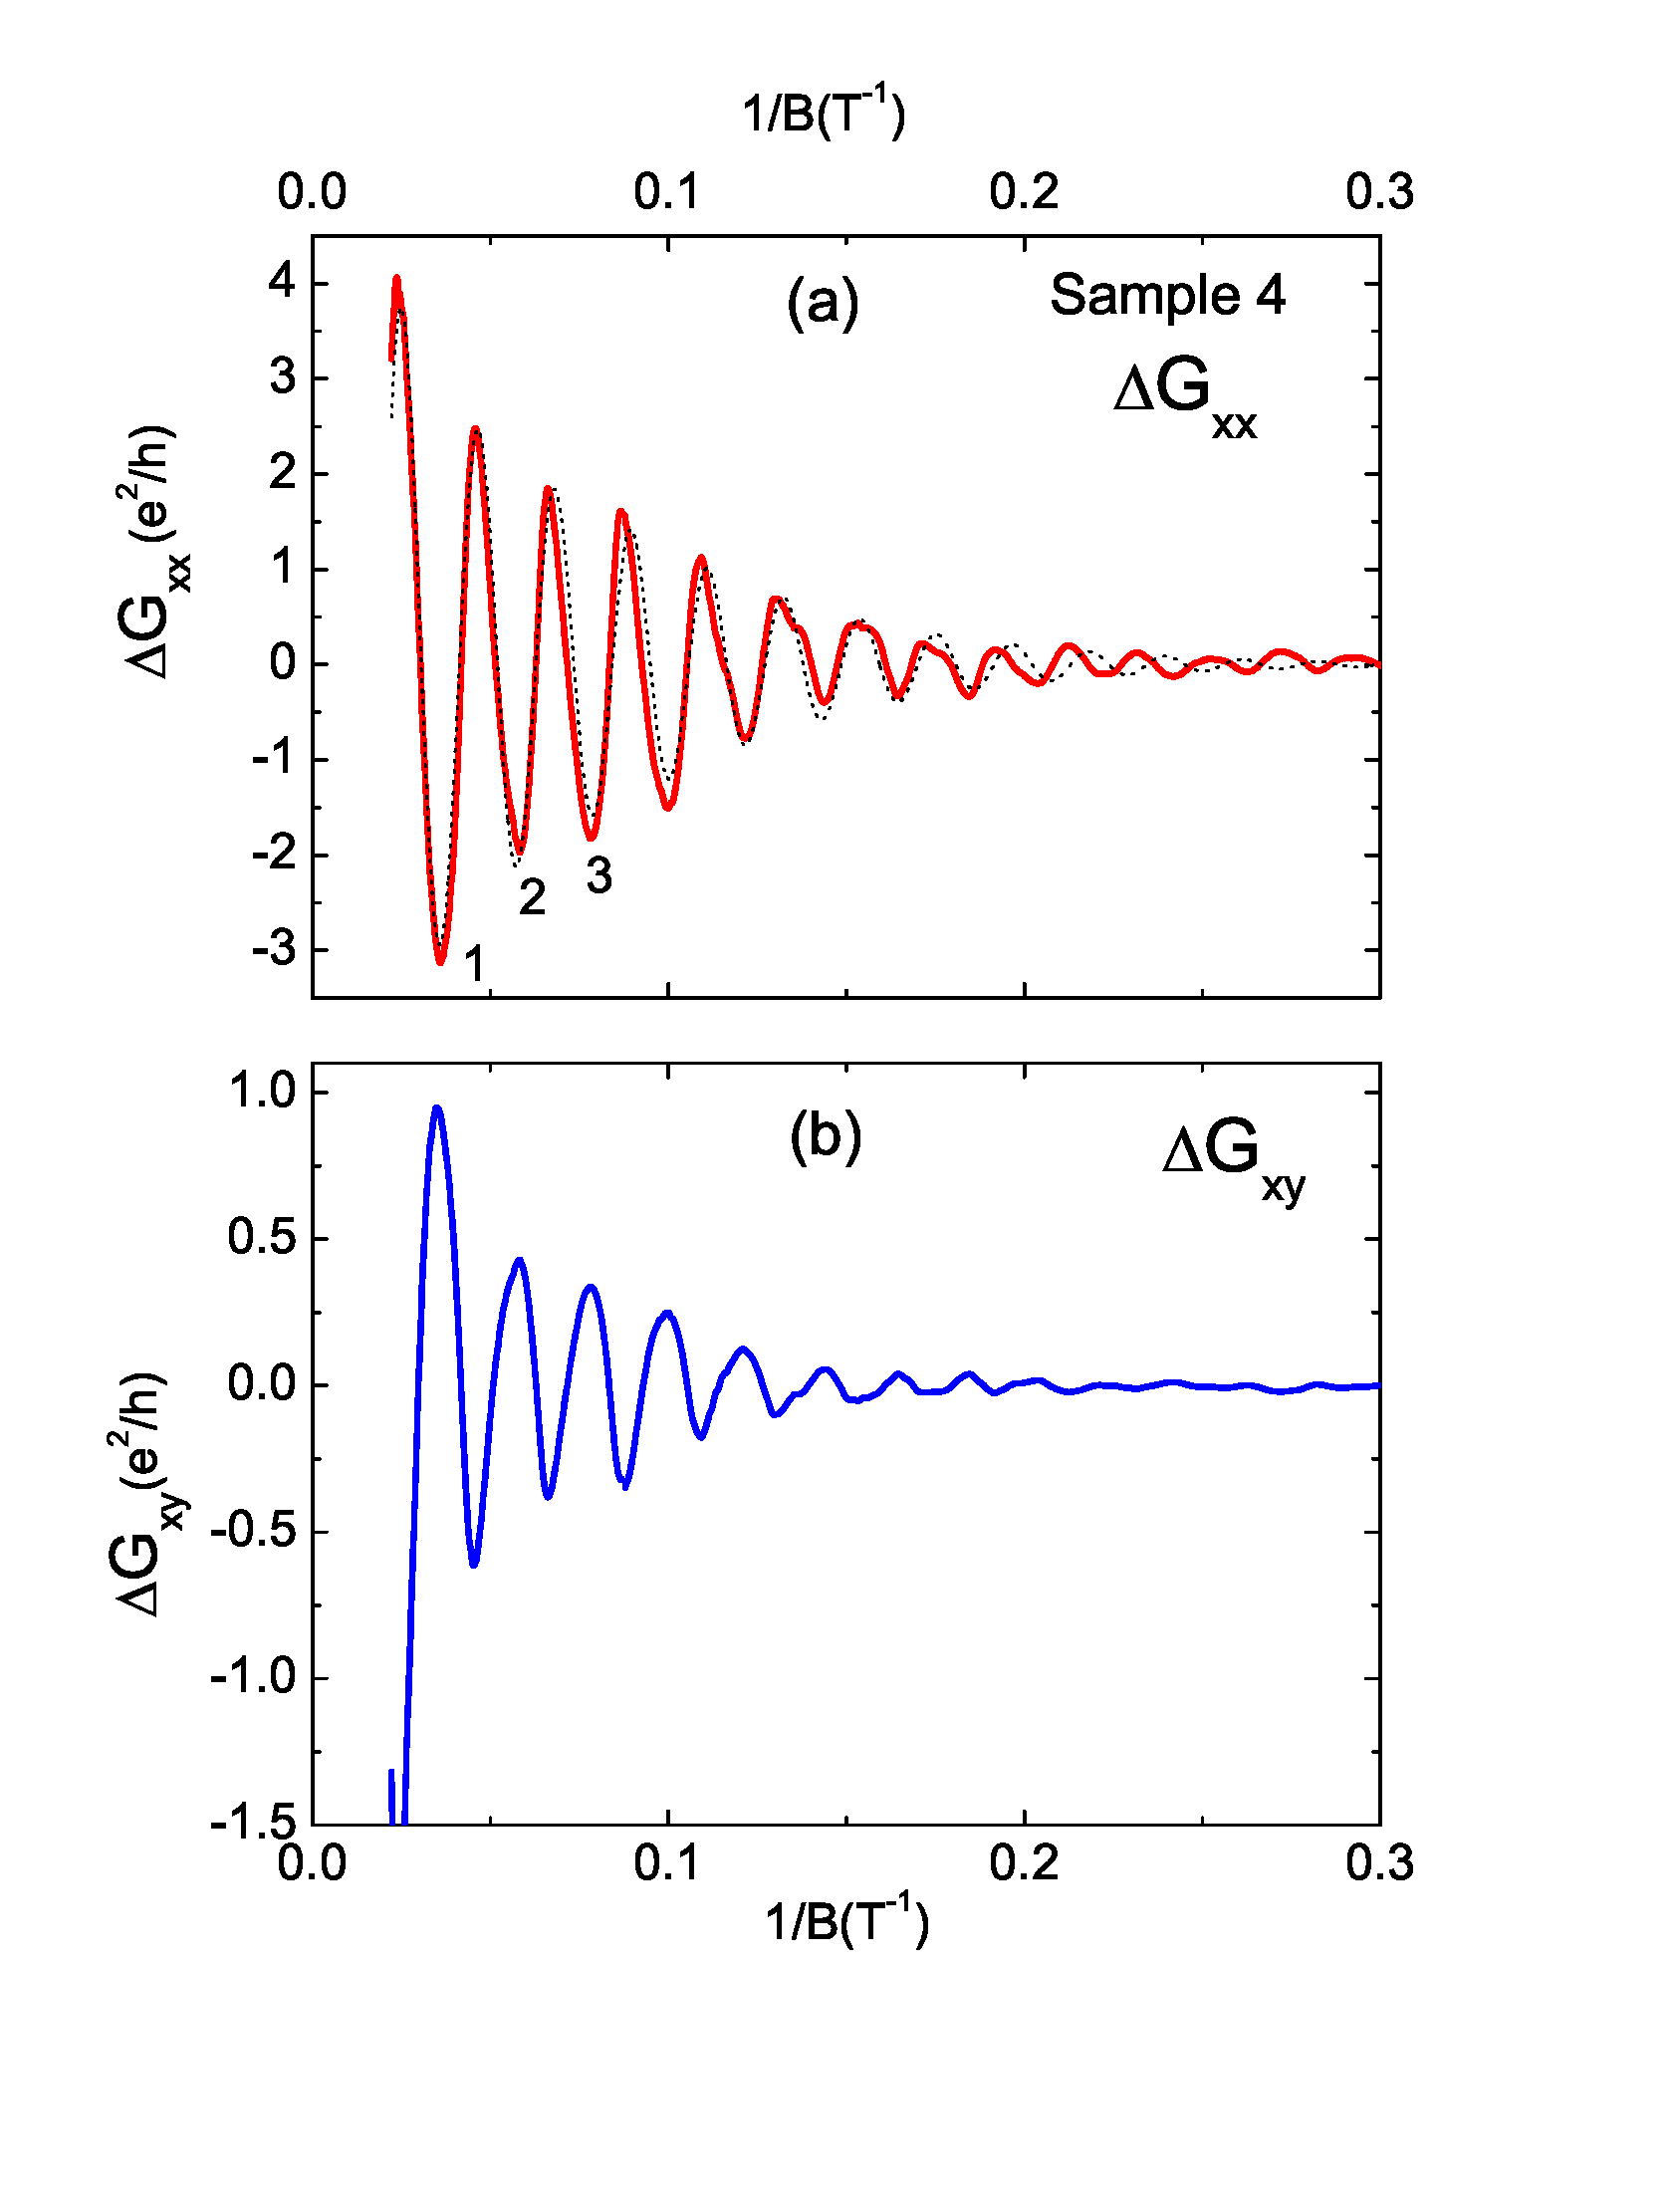
\includegraphics[width=0.8\linewidth]{ch-bts/figures/FigDG.eps}
\caption{\label{figG} (color online)
The oscillatory component of the conductance $\Delta G_{xx}$ (Panel a) and the 
Hall conductance $\Delta G_{xy}$ (Panel b) after a background subtraction in Sample 4 plotted against $1/B$ ($T$ = 0.7 K). The two quantities
are normalized to $e^2/h$. In Panel a, the faint dashed curve is a fit 
to the Lifshitz-Kosevich expression (Eq. \ref{eq:sdh}) using a single frequency. The fit is very good at high field but there is a phase shift at low $B$. The fitting parameters yield a surface mobility of 3,200$\pm$300 cm$^2$/Vs, with $k_F\ell$ = 30. This mobility is higher than that in our 14T experiment. Through the Fermi wavevector $k_F$ and the mobility from the fit, we can calculate $G^s$ in Sample 4 and it accounts for $\sim 19\%$ of the total conductance at 4 K. And at the highest field, the surface state has entered the $n$=1 LL, which could give us a precise measurement of the Berry phase.
The LL indices $n$ = 1,2,3 are indicated for the 
minima of $\Delta G_{xx}$. 
}
  \end{center}
\end{figure}

%%%%%%%%%%%%%%%%%%%%%%%%%%%%%%%%%%
\subsection{Quantum oscillations up to 45T}

The transport measurement results up to 45 T in Samples 1 and 4 are discussed below (in which $R_H$ = -137 and -52 cm$^3$/C, respectively, at 4 K). As shown in Fig. \ref{figRvsB}a, we have observed large and well-resolved SdH oscillations in these samples. Such distinguishable surface quantum oscillations allow us to investigate the interesting problems in the quantum limit with the best accuracy. As displayed in Fig. \ref{figRvsB}a, the peak-to-peak SdH amplitudes in the longitudinal resistance $R_{xx}$ in Sample 4 grows with $B$ and eventually accounts for $\sim$17$\%$ of the total resistance at 45T. Since the oscillations purely come from the surface states, it indicates that the surface contribution is comparable to the bulk current in our samples. To determine $B_n$ accurately, it is appropriate to convert $R_{ij}$ to the conductance matrix by $G_{xx} = R_{xx}/[R_{xx}^2+R_{yx}^2]$ and $G_{xy}= R_{yx}/[R_{xx}^2+R_{yx}^2]$. A display of $G_{xy}$ is in Fig. \ref{figRvsB}b. Then we also need to subtract an appropriate background to isolate the oscillatory part and determine the accurate positions of the \emph{minima} and \emph{maxima} of  $G_{xx}$. We first use a smooth polynomial function to fit the envelope of the oscillations (the faint dashed curves in Fig. \ref{figRvsB}), and then locate the midpoints between the two envelope curves to define the background curve.


After removing the background, we present the oscillatory components $\Delta G_{xx}$ and $\Delta G_{xy}$ versus $1/B$ in Fig. \ref{figG}a and \ref{figG}b respectively (both are normalized to the quantum of conductance $e^2/h$).
In Panel (a), we have also added a fit to the standard Lifshitz-Kosevich expression (Eq. \ref{eq:sdh}) with just
one frequency (dashed curve). The fit is very good at high field but there is a phase shift at low $B$. The fitting parameters yield a surface mobility of 3,200 cm$^2$/Vs and a metallicity parameter $k_F\ell$ = 30. This mobility is higher than that in our 14T experiment. We will discuss the interesting phase shift apparent at low $B$ later.


%%%%%%%%%%%%%%%%%%%%%%%%%%%%%%%%%%
%%%%%%%%%%%%%%%%%%%%%%%%%%%%%%%%%%
%%%%%%%%%%%%%%%%%%%%%%%%%%%%%%%%%% FIGURE 4
\begin{figure}[!htbp]
  \begin{center}
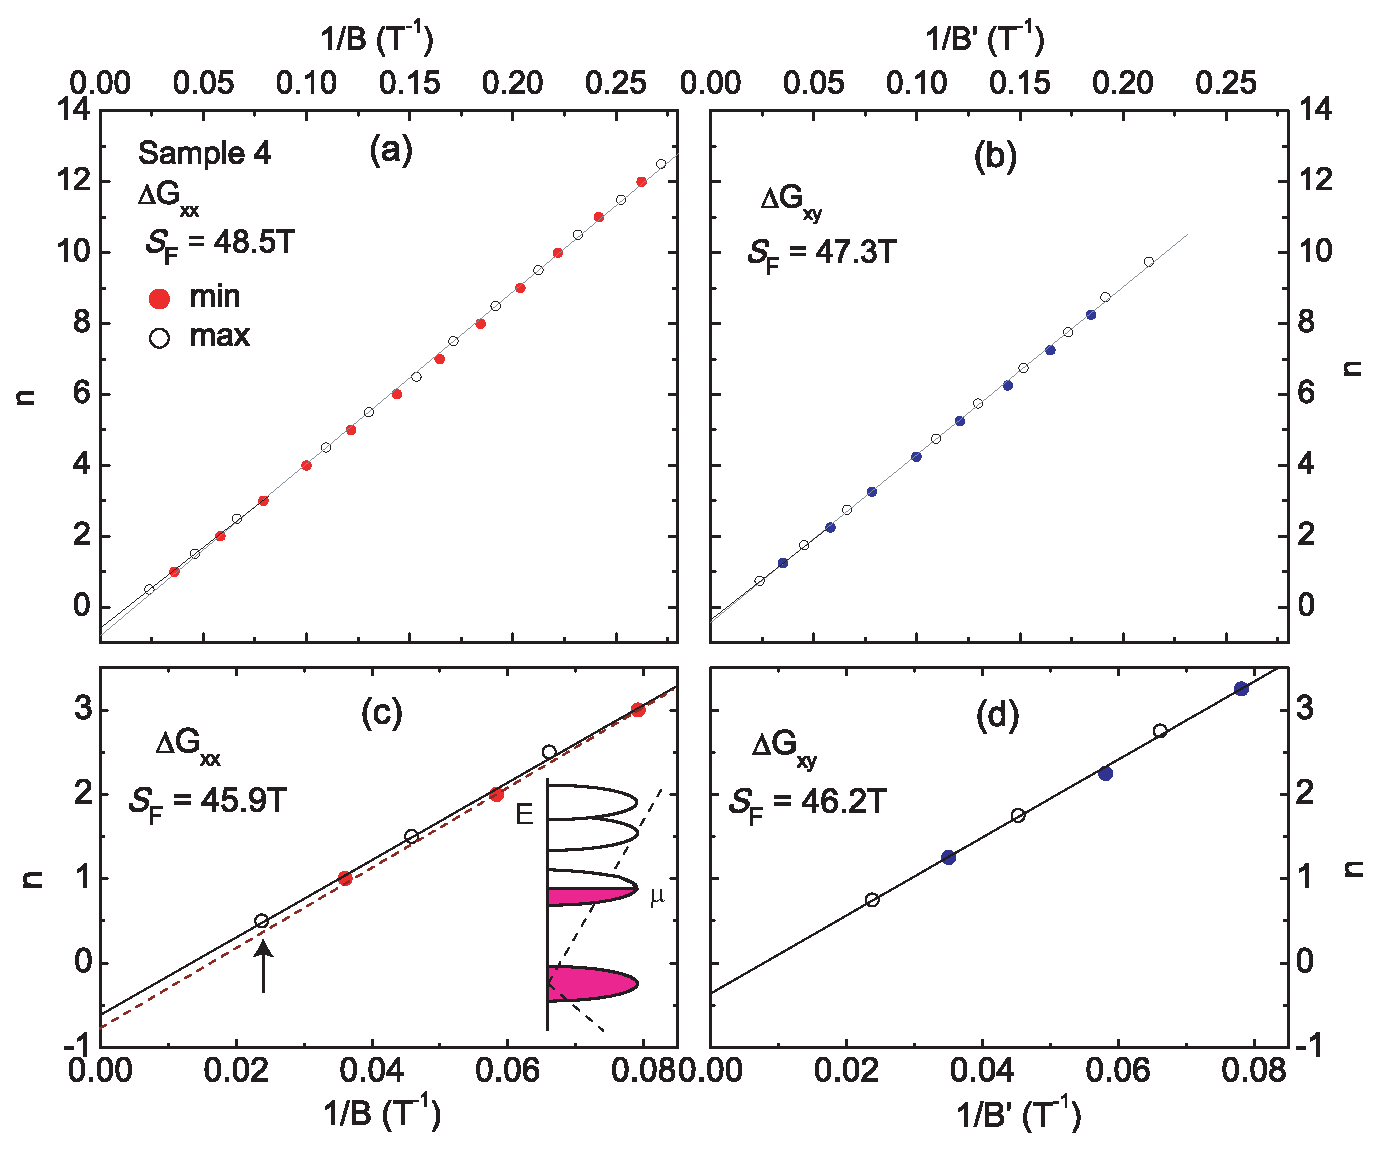
\includegraphics[width=0.9\linewidth]{ch-bts/figures/FigIndexAll4.eps}
\caption{\label{figindex} (color online)
The index plots of $1/B_n$ \emph{vs.} the integers $n$ in Sample 4. In Panel (a), $B_n$ is obtained from
the minima of $\Delta G_{xx}$. In Panel (b), the index field $B'_n$ is inferred from the minima of
$-\Delta G_{xy}$. $B'_n$ is plotted against $n+\frac14$, where the $\frac14$ shift arises because 
the minima in $d\Delta G_{xy}/dB$
align with the minima in $\Delta G_{xx}$. We expand the scale in Panels (c) and (d) to
show the intercepts more clearly. 
In Panel (c), the solid straight line is the best fit to the extrema fields for $n\le$3. The
dashed line is the best fit to all the extrema field shown in Panel (a).
The sketch shows the chemical potential $\mu$ in relation to the filled LLs (solid color) in the Dirac spectrum when
$B$ = 42.0 T (arrow). 
}
  \end{center}
\end{figure}

%%%%%%%%%%%%%%%%%%%%%%%%%%%%%%%%%%

Then we can use our above criteria to determine $B_n$, and Figure \ref{figindex}a exhibits the minima 
of $\Delta G_{xx}$ versus $n$ (solid circles) of Sample 4. In addition, the maxima of $\Delta G_{xx}$ have been plotted as open circles (shifted by $\frac12$) and they correspond to $n+\frac12$. The slope of the fitted straight line gives a Fermi cross-section area $S_F$ of 48.5 T.
A similar plot based on the extrema of the Hall conductance $\Delta G_{xy}$ 
is shown in Fig. \ref{figindex}b. As in the quantum Hall system, the $G_{xy}$ and $G_{xx}$ extrema have a $\frac{\pi}{2}$ phase difference, and thus the minima in $-\Delta G_{xy}$ correspond to $n+\frac14$.The Fermi surface area $S_F$ found from $\Delta G_{xy}$ (47.3 T) is consistent with the value from  $\Delta G_{xx}$ within our resolution. We also note the values of $n$ = 1,2,3 at the minima of $\Delta G_{xx}$ in Fig. \ref{figG}a.


In order to have a clear view of the intercept $\gamma$, we expand the scale in Fig. \ref{figindex}c. The best-fit straight line passing through the six extrema of $\Delta G_{xx}$ intercepts the $n$-axis at the value $\gamma$ = -0.61$\pm$0.03. Similarly, the high-field
extrema of $\Delta G_{xy}$ and their fitted line are presented in Fig. \ref{figindex}d. The intercept occurs at $\gamma$ = -0.37$\pm$0.03. Within our uncertainties, both values are significantly closer to the theoretical value $\gamma=-\frac12$ than 0 or 1. Also, our samples have already entered the $n=\frac12$ Landau level, it is significantly closer to the limit $1/B\to 0$ than previous experiments. As a result, it can also give a better resolution in determining the intercept $\gamma$. Hence, the high-field results we present here provide clear transport evidence for a Dirac spectrum of the surface states on Bi$_2$Te$_2$Se.

Another interesting thing is the large amplitudes of the quantum oscillations. Although we have not observed any quantized Hall steps in Fig. \ref{figG}b (the oscillatory component that we extract by subtracting a smooth background from the bulk states), we find that the peak-to-peak
amplitude of $\Delta G_{xy}$ at $n=1$ is $\sim$0.8 $e^2/h$ per surface, which is of the order
of the quantized Hall conductance value.

In Sample 1, the amplitudes of the observed SdH oscillations are considerably
weaker (Fig. \ref{figG1}a) than those of Sample 4. But it also enters the $n=1$ Landau level at the highest field. The fitted straight line to the $1/B_n$ vs. $n$ plot also intercepts the $n$-axis at $\gamma$ = -0.45$\pm$0.02, confirming a Dirac spectrum in Sample 1's surface states.

In the expanded plot Fig. \ref{figindex}c we show why the high fields are necessary to find $\gamma$ accurately. At a field as high as 45T, we can access the very low Landau index as $n=\frac12$ in Figs. \ref{figindex}c and d. Thus the bias and uncertainty that the fitted intercept can have is reduced considerably because it is almost fixed by the experimental data at $n=\frac12$. In our data, an intercept $\gamma = 0$ can be safely excluded as the allowed error from our fit is small. A more subtle point is the slight curvature of the index plot. In Fig. \ref{figindex}c, if we extrapolate the best-fit line (dashed) using the total data set from 3 to 45 T, its intercept yields -0.78, nearly exactly between -1 and
-$\frac12$. In comparison, the best-fit line (bold) to the high-field extrema
for $n\le$3 yields an intercept (-0.61) closer to -$\frac12$. This difference implies that the index curve
$1/B_n$ vs. $n$ develops a slight curvature over the large field range. And as we may notice in Fig. \ref{figG}a, this curvature may also appear as a phase shift at different fields when it is compared to the single-frequency fit. 


%%%%%%%%%%%%%%%%%%%%%%%%%%%%%%%%%%
%%%%%%%%%%%%%%%%%%%%%%%%%%%%%%%%%%
%%%%%%%%%%%%%%%%%%%%%%%%%%%%%%%%%% FIGURE 5
\begin{figure}[!htbp]
  \begin{center}
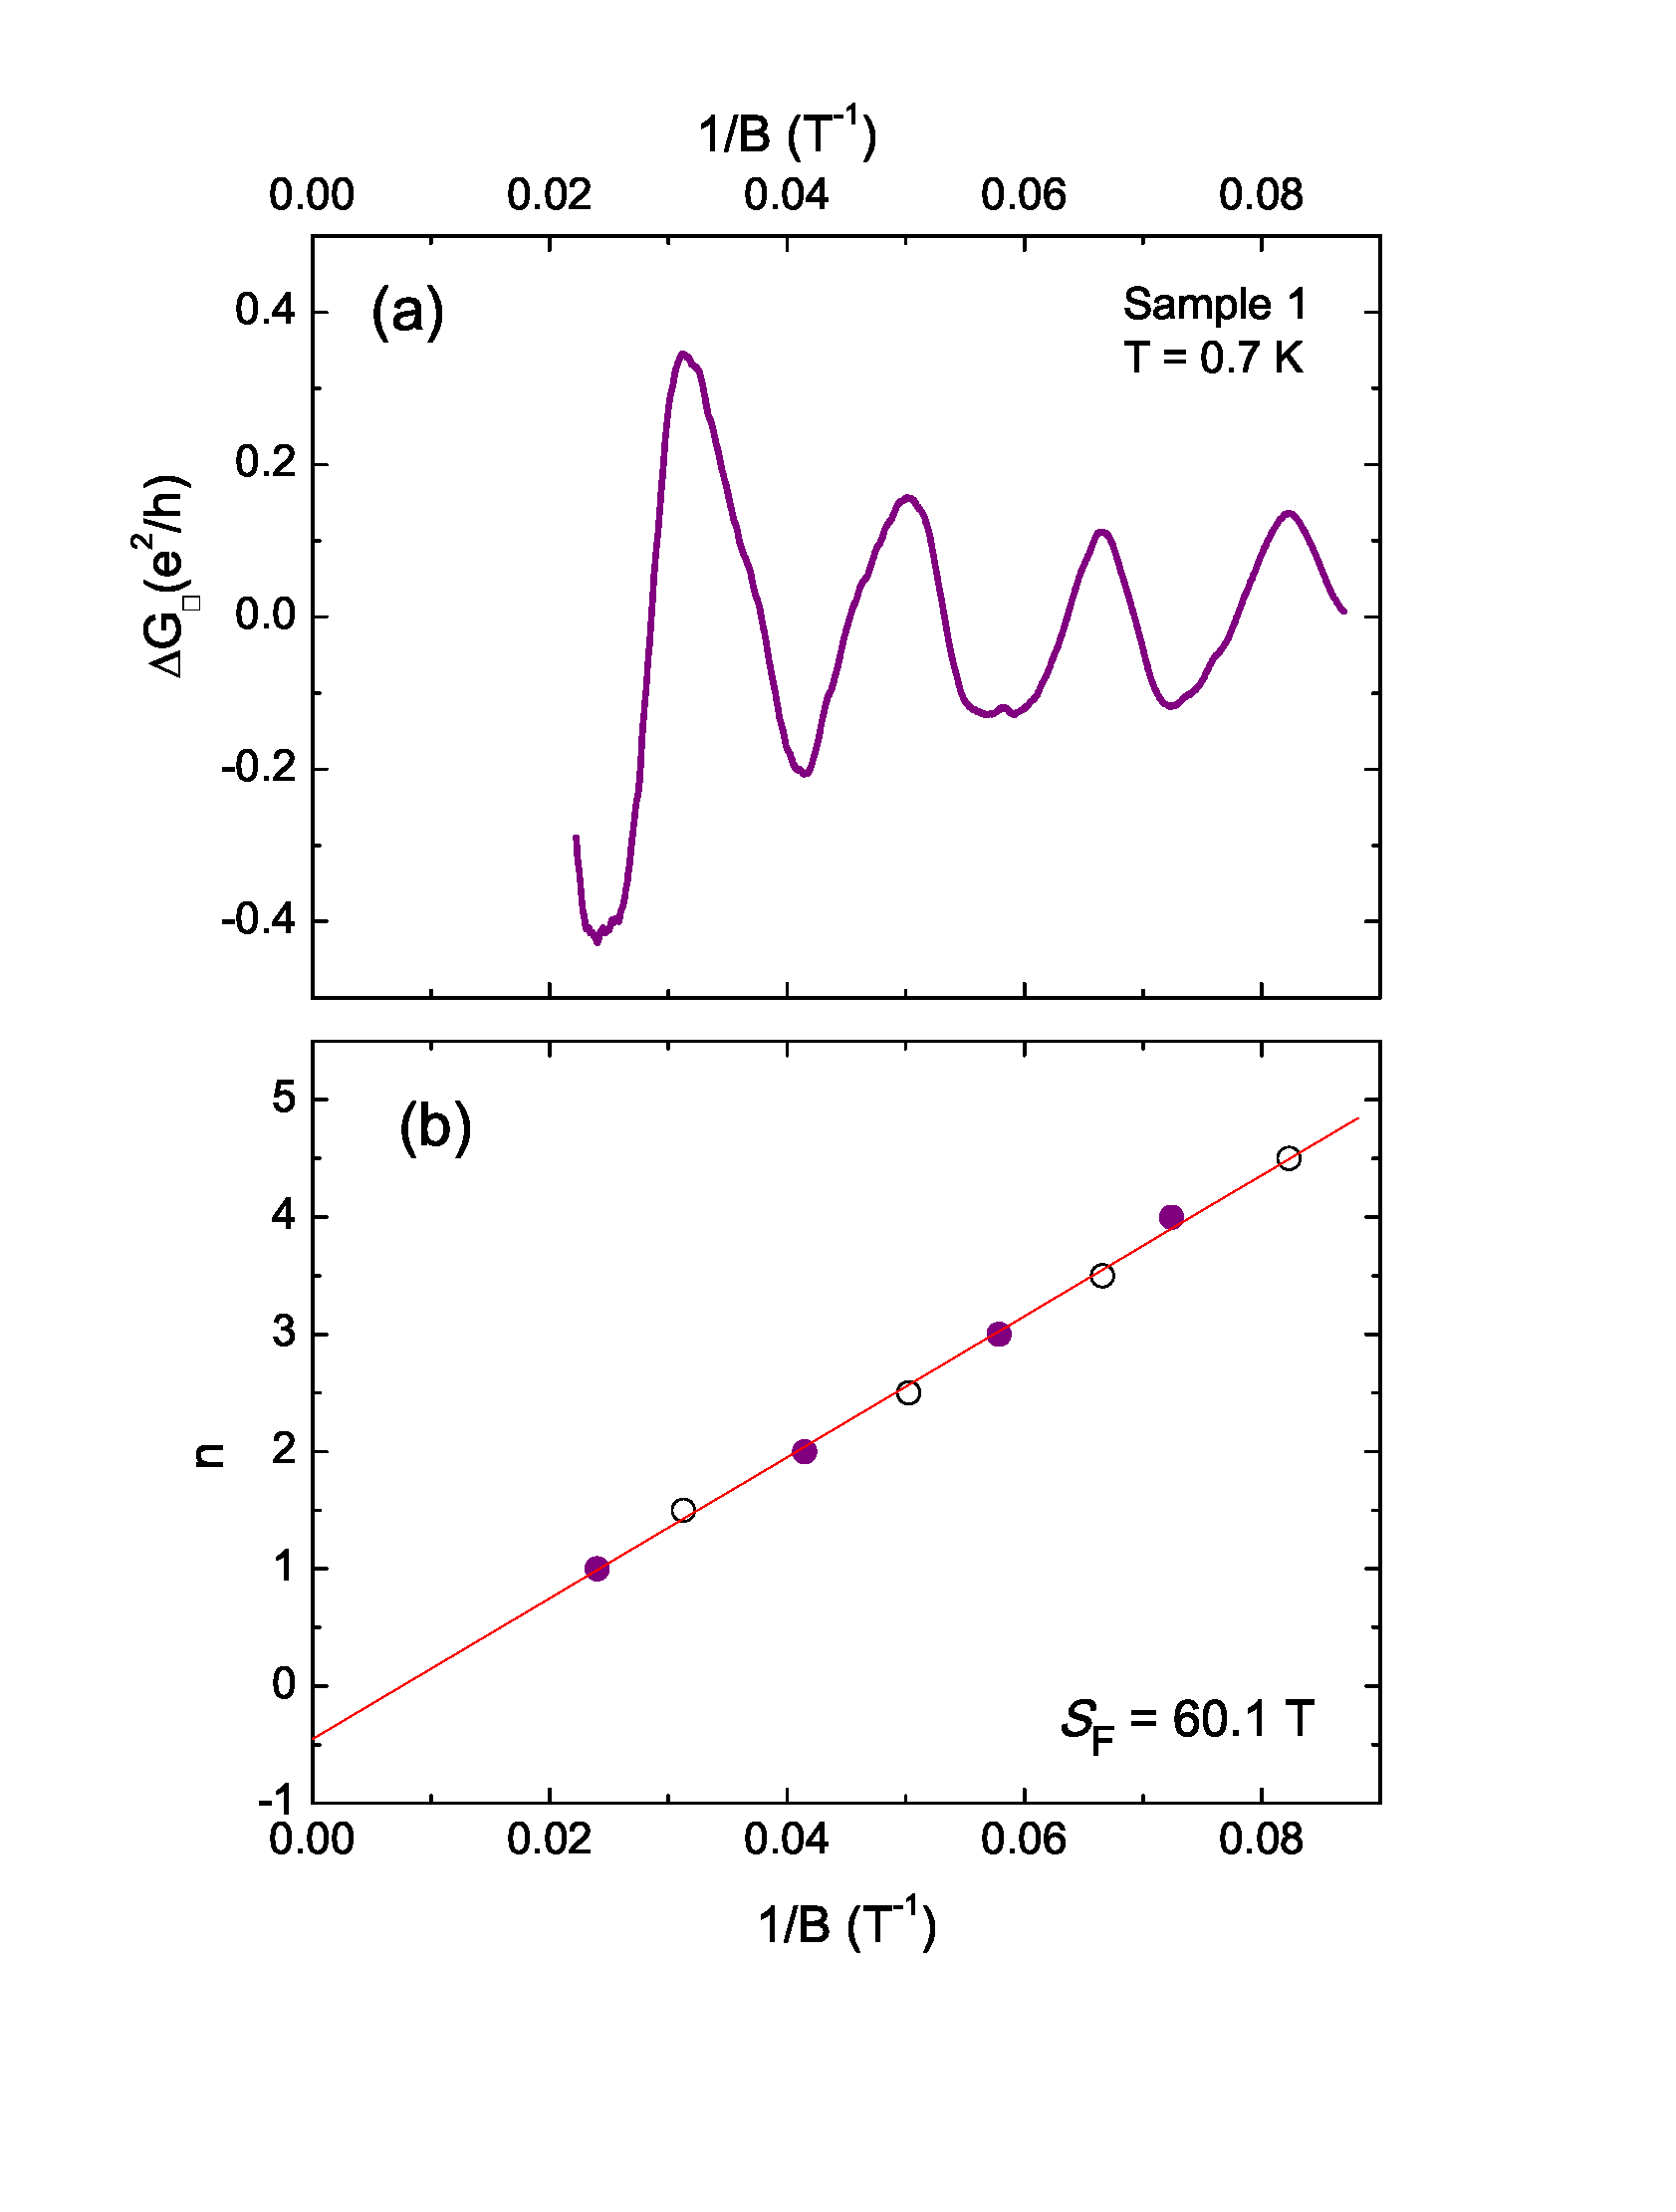
\includegraphics[width=0.9\linewidth]{ch-bts/figures/FigGindexS1.eps}
\caption{\label{figG1} 
The oscillatory component $\Delta G_{xx}$ vs. $1/B$ (Panel a) and the 
index plot of $1/B_n$ vs. $n$ (Panel b) in Sample 1. The intercept $\gamma$ of the best-fit line 
is -0.45$\pm$0.02.}
  \end{center}
\end{figure}

%%%%%%%%%%%%%%%%%%%%%%%%%%%%%%%%%%
%A second issue we address is the strength of the Zeeman energy.
%Strict particle-hole symmetry implies that it is unshifted in energy. 
%On the other hand, a large Zeeman energy $g\mu_BB$ may lead to high-field distortion of the
%SdH period ($g$ is the surface Lande g-factor
%and $\mu_B$ the Bohr magneton).
%The in-field STM experiments ~\cite{Hanaguri,Xue10} have shown that the $n$ = 0 LL is unshifted up to 11 Tesla. 
%This test can be extended to much larger $B$ in transport experiments, but early SdH experiments had limited
%resolution~\cite{Qu,Analytis}. Values of $g$ as large as 76 have been inferred from low-field
%SdH oscillations in Bi$_2$Te$_2$Se~\cite{Taskin}.

As discussed above, the Zeeman energy could possibly cause a curvature in the index plot. When the Zeeman term is included, the Hamiltonian is
\be
H = v_F {\bf \hat{n}}\cdot \bm{\sigma\times\pi}- \frac{g\mu_B}{2} {\bf B}\cdot\bm{\sigma}
\label{eq:H}
\ee
where $\bf \hat{n}$ is the unit vector normal to the surface. $\bm\sigma$ are the spin Pauli matrices, and $\bm{\pi} = {\bf p}-e{\bf A}$ is the momentum $\bf p$ of the
electron in a vector potential ${\bf A}$. The LL energy is given by 
\be 
E_n = \pm\sqrt{2n\hbar v_F^2 eB + (g\mu_B B/2)^2}.
\label{eq:En}
\ee
In contrast to the case without Zeeman energy, the energy of the $n=0$ LL increases linearly with $B$ instead of being unshifted.
For a large $g$-factor, the $1/B_n$ vs. $n$ curve will deviate from a straight line as $1/B\to$ 0. However, in our experiment, we have
tracked the LLs to $n$ = 1. The weak deviation from a straight line in Fig. \ref{figindex}c) 
is inconsistent with values of $g$ substantially larger than 2. More importantly, the
observed curvature is opposite in sign to that predicted by Eq. \ref{eq:En}. Since there is no significant deviation in our data that could be explained by the Zeeman energy, we conclude that the 
the $g$ factor of the surface states in Bi$_2$Te$_2$Se is not significantly greater than 2 in the quantum limit. 

\subsection{Surface carrier mobility}\label{fit}

In most of the Bi-based topological compounds, it is very difficult to separate $G^s$ from $G^b$ reliably.  
But Shubnikov de-Haas (SdH) oscillations -- when measured with a high resolution -- 
provide a powerful way to isolate the surface conductance.
The period of the oscillations yields the Fermi surface area and thus the Fermi wavevector $k_F$. The surface mobility and the scattering rate can also be obtained by fitting the field dependence of the SdH amplitudes.
Then we can obtain the zero-field value of $G^s_{xx}\equiv G^s$ using
\be
G^s = (e^2/h)k_F\ell.
\label{eq:Gs}
\ee

To isolate the surface quantum oscillations, we first use a smooth polynomial function to simulate the envelope curves
passing through the extrema of the oscillations on the raw data curves as explained above. The background is defined as the midpoints of the two envelope curves. Then we obtain the oscillatory component $\Delta G_{xx}$ by subtracting the background from $G_{xx}$. We also notice that  $\Delta G_{xx}$ may not account for all of the
surface conductance, because its field-averaged value $\langle\Delta G_{xx}\rangle_B$
vanishes while $G^s_{xx}$ should have some field dependence. Hence we conclude that $\Delta G_{xx}$ is smaller than $G^s_{xx}$.



%%%%%%%%%%%%%%%%%%%%%%%%%%%%%%%%%%%%%%%%
%%%%%%%%%%%%%%%%%%%%%%%%%%%%%%%%%%%%%%%%
%%%%%%%%%%%%%%%%%%%%%%%%%%%%%%%%%%%%%%%%
%%%%%%%%%%%%%%%%%%%%%%%%%%%%%%%%%%%%%%%% FIGURE 6

\begin{figure}[!htbp]
  \begin{center}   
\incl[width=0.9\linewidth]{ch-bts/figures/FigGfit.eps} 
\caption{\label{figfit} 
The oscillatory component of the conductance $\Delta G_{xx}$ in Sample 4 at 0.7 K
(solid curve) and the fit to Eq. \ref{eq:sdh} using only one frequency (dashed curve). 
}
  \end{center}
\efig

Then we leveraged the standard Lifshitz-Kosevich expression~\cite{Roth} to fit the oscillatory component $\Delta G_{xx}$. The formula is:
\be
\frac{\Delta G_{xx}}{G_{xx}} = \left(\frac{\hbar\omega_c}{2E_F}\right)^{\frac12}
\frac{\lambda}{\sinh\lambda} e^{-\lambda_D}\cos
\left[\frac{2\pi E_F}{\hbar\omega_c}+\varphi\right],
\label{eq:sdh}
\ee
%with $\lambda = 2\pi^2k_BT/\hbar\omega_c$ and $\lambda_D = 2\pi^2k_BT_D/\hbar\omega_c$,
%where $\omega_c$ is the cyclotron frequency and 
%the Dingle temperature is given by $T_D = \hbar/(2\pi k_B\tau)$,
%with $\tau$ the lifetime. For 2D Dirac electrons, the SdH frequency is determined by the chemical potential as
%$2\pi E_FB/(\hbar\omega_c)$, which simplifies to $4\pi^2\hbar n_s/e$, with the 2D
%carrier density $n_s = k_F^2/4\pi$ (per spin).  
%In equation \ref{eq:sdh}, the cyclotron mass for a Dirac system is given by $m_c = E/v_F^2$.  
The formula is almost the same as Eq. \ref{eq:sdh_hall} except that the phase $\varphi$ here is shifted by $\frac{\pi}{2}$ from that of the Hall conductivity. 


As displayed in Fig. \ref{figfit}, with one Fermi pocket, we have already obtained a very good fit (dashed line) to the observed oscillations (bold curve). The three fitting parameters are $k_F$ = 0.038 \AA$^{-1}$, $\varphi$ = 0.65$\pi$ and
$T_D$ = 8.5$\pm$1.5 K. They imply a surface 
mean-free-path $\ell$ = 79$\pm$8 nm and mobility $\mu_s = e\ell/\hbar k_F$ = 3,200$\pm$300 cm$^2$/Vs.
The metallicity parameter $k_F\ell$ equals 30. 
These parameters indicate that, in Sample 4 at $B$=0, $G^s$ accounts for $\sim 19\%$ of the
total observed conductance.
The parameters here are also similar to those obtained from our earlier
sample in the 14T experiment, which had a slightly larger $k_F$ (0.047 \AA$^{-1}$)~\cite{Xiong2012}. 


Again, the mobility from the SdH oscillations provides a strong, quantitative argument that the SdH oscillations
origin from surface states. Otherwise if the oscillations arise 
from the bulk states, the SdH period gives a 3D Fermi sphere 
of radius $k_F$ = 0.038 \AA$^{-1}$, or equivalently a 3D carrier density of 1.86$\times 10^{18}$ cm$^{-3}$.  With
this density and the mobility inferred by the Lifshitz-Kosevich formula Eq. \ref{eq:sdh}, we can obtain a 3D resistivity $\rho_b \sim$ 1.1 m$\Omega$cm at 4 K. Instead our measured $\rho$ is around 5 $\Omega$cm, a factor of 4,500 different from the 3D one. Such a large difference eliminates the possibility of the bulk origin of the quantum oscillations.


%\subsection{Discussions}
%
%Many non-trivial properties of the Dirac-like topological surface states have been investigated by the surface sensitive ARPES and STM experiments. Here we showed that these surface states may also display interesting physics for the transport experiments at high magnetic fields. Although the large amount of bulk carriers may overwhelm the fragile surface states on TI, with the appropriate charge compensation method and a high magnetic field, we can use the powerful SdH oscillations to identify the surface conductance and explore the surface states' properties such as $k_F\ell$ and the mobility. With a magnetic field up to 45T, our Bi$_2$Te$_2$Se samples could access $n$=1 or lower Landau levels, providing an accurate determination of the intercept $\gamma$. The intercept we obtained by linearly fitting the Landau index plot $n$ versus $1/B_n$ is close to $-\frac12$. It corresponds to a non-trivial $\pi$ Berry phase expected for the Dirac dispersion of the surface states on TI.  
%
%We also hope to emphasize that the appropriate definition of $B_n$ should be applied to exclude any mistakes in identifying $\gamma$. As explained in the above sections, $B_n$ should be identified with minima in $G_{xx}$ or maxima in $R_{xx}$ when the bulk conductance dominate. In fact it is very tempting to isolate oscillatory $\Delta R_{xx}$ by subtracting a smooth background and then assign integer indices to the minima of the $\Delta R_{xx}$. Nevertheless, this way will result in an opposite and wrong definition of the index. Then it will yield a fake $\frac12$-shift in the intercept even for Schr\"{o}dinger electrons. Furthermore it needs a low index to significantly reduce the uncertainties in fixing $\gamma$. An index plot with many but large indices may still have a large error bar in determining $\gamma$ as the curvature in the plot could easily change the intercept obtained by extrapolation. 
%
%The linearity of the index plot in Figs. \ref{figindex} and \ref{figG1} show that the Lande
%$g$-factor can not be large ($g\sim$2). The $n$ = 0 LL is unshifted even at 45 T, consistent with 
%STM experiments taken at 11 T~\cite{Hanaguri,Xue10}.
%
%Finally, we hope to add some comments on the results in the large-$B$ limit.
%In Fig. \ref{figG}a, the last maximum in $\Delta G_{xx}$ (at $B\simeq$ 40 T) corresponds to
%$n$ = $\frac12$ (see arrow in the index plot in Fig. \ref{figindex}c). At this field, the
%Fermi energy $E_F$ is aligned with the center of the $n$ = 1 LL, as sketched in the
%inset in Fig. \ref{figindex}c. According to our indexing scheme, it means that there are two half-filled
%LLs between $E_F$ and the Dirac Point, with $\frac12$ of the $n=1$ Landau level and $\frac12$ 
%from the unshifted LL at the Dirac Point. Since there are not many LLs between $E_F$ and the Dirac point, our high-field results provide 
%rather firm evidence 
%for this $\frac12$-shift in the limit $1/B\to 0$. 
%As the inset in Fig. \ref{figindex}c implies, we may be able to reach the interesting
%states in the $n$ = 0 LL in Bi$_2$Te$_2$Se in fields higher than 45 T. 

\section{Discussions and Summary}
\label{sec:bts:summary}


Many non-trivial properties of the Dirac-like topological surface states have been investigated by the surface sensitive ARPES and STM experiments. Although the large amount of bulk carriers may overwhelm the fragile surface states on many TIs, here we found a TI crystal with a large bulk resistivity with the appropriate charge compensation method. The suppressed bulk conductance has enabled us to measure the surface states of Bi$_2$Te$_2$Se directly in a transport experiment. We showed that these surface states on Bi$_2$Te$_2$Se may also display interesting physics for the transport experiments at high magnetic fields. We can use the powerful SdH oscillations to identify the surface conductance and explore the surface states' properties such as $k_F\ell$ and the mobility. With a magnetic field up to 45T, our Bi$_2$Te$_2$Se samples could access $n$=1 or lower Landau levels, providing an accurate determination of the intercept $\gamma$. The intercept we obtained by linearly fitting the Landau index plot $n$ versus $1/B_n$ is close to $-\frac12$. It corresponds to a non-trivial $\pi$ Berry phase expected for the Dirac dispersion of the surface states on TI.  

We also hope to emphasize that the appropriate definition of $B_n$ should be applied to exclude any mistakes in identifying $\gamma$. As explained in the above sections, $B_n$ should be identified with minima in $G_{xx}$ or maxima in $R_{xx}$ when the bulk conductance dominate. In fact it is very tempting to isolate oscillatory $\Delta R_{xx}$ by subtracting a smooth background and then assign integer indices to the minima of the $\Delta R_{xx}$. Nevertheless, this way will result in an opposite and wrong definition of the index. Then it will yield a fake $\frac12$-shift in the intercept even for Schr\"{o}dinger electrons. Furthermore it needs a low index to significantly reduce the uncertainties in fixing $\gamma$. An index plot with many but large indices may still have a large error bar in determining $\gamma$ as the curvature in the plot could easily change the intercept obtained by extrapolation. 

The linearity of the index plot in Figs. \ref{figindex} and \ref{figG1} show that the Lande
$g$-factor can not be large ($g\sim$2). The $n$ = 0 LL is unshifted even at 45 T, consistent with 
STM experiments taken at 11 T~\cite{Hanaguri,Xue10}.

Finally, we hope to add some comments on the results in the large-$B$ limit.
In Fig. \ref{figG}a, the last maximum in $\Delta G_{xx}$ (at $B\simeq$ 40 T) corresponds to
$n$ = $\frac12$ (see arrow in the index plot in Fig. \ref{figindex}c). At this field, the
Fermi energy $E_F$ is aligned with the center of the $n$ = 1 LL, as sketched in the
inset in Fig. \ref{figindex}c. According to our indexing scheme, it means that there are two half-filled
LLs between $E_F$ and the Dirac Point, with $\frac12$ of the $n=1$ Landau level and $\frac12$ 
from the unshifted LL at the Dirac Point. Since there are not many LLs between $E_F$ and the Dirac point, our high-field results provide 
rather firm evidence 
for this $\frac12$-shift in the limit $1/B\to 0$. 
As the inset in Fig. \ref{figindex}c implies, we may be able to reach the interesting
states in the $n$ = 0 LL in Bi$_2$Te$_2$Se in fields higher than 45 T. 

